\documentclass{article}
\usepackage[utf8]{inputenc}
\usepackage[super,square]{natbib}
\usepackage{tabularx}
\usepackage{parskip}
\usepackage[margin=1.4in]{geometry}
\usepackage{csquotes}
\usepackage{amsmath}
\usepackage{amsfonts}
\usepackage{amsthm}
\usepackage{graphicx}
\usepackage{float}
\usepackage{hyperref}


\newcommand{\comment}[1]{}
\numberwithin{equation}{section}

\title{\vspace{-3cm} Statistical Learning Notes (ISLR)}
\author{}
\date{}

\comment{
- https://www.dataschool.io/15-hours-of-expert-machine-learning-videos/
- https://github.com/tdpetrou/Machine-Learning-Books-With-Python

Outline:
- Go over statistical learning book and add code snippets with python scikit learn
- Go over VC theory paper
- Add definition in margin https://tex.stackexchange.com/questions/518603/theorem-and-definition-name-in-margin

2: Basics of stat learning and K Nearest Neighbor
3: Linear Regression
4: Logistic Regression and Linear Discriminant Analysis
5: Crossvalidation and bootstrapping
6: Regression improvements - stepwise regression, regularized regression and others
7: Non-linear methods - Polynomial regression, splines, general additive models
8: Decision Trees and Random Forests - bagging/boosting
9: Support Vector Machines
10: Unsupervised Learning- Principal components analysis and clustering
}

\begin{document}
\maketitle
\vspace{-1.5cm}

\tableofcontents
\newpage

\section{Introduction}
\subsection{A Brief History of Statistical Learning}
    \begin{enumerate}
        \item  At the beginning of the nineteenth century, Legendre and Gauss published papers on the method of least squares, which implemented the earliest form of what is now known as linear regression.
        \item In 1936 Fisher proposed linear discriminant analysis.
        \item In the 1940s, various authors put forth an alternative approach, logistic regression.
        \item In the 1950's, Frank Rosenblatt introduced the Perceptron and Neural Networks.
        \item In the 1960's, various authors introduced Nearest Neighbor and K-means clustering.
        \item In the early 1970s, Nelder and Wedderburn coined the term generalized linear models for an entire class of statistical learning methods that include both linear and logistic regression as special cases.
        \item By the end of the 1970s, many more techniques for learning from data were available but all were almost all linear because of computational limitations.
        \item By the 1980s, computing technology had finally improved sufficiently that non-linear methods were no longer computationally prohibitive.
        \item In the mid 1980s, Breiman, Friedman, Olshen and Stone introduced classification and regression trees,  including cross-validation for model selection.
        \item In 1986,  Hastie and Tibshirani introduced generalized additive models for a class of non-linear extensions to generalized linear models.
        \item In the 1990's, Vapnik introduced Support Vector Machines.
        \item In the 2000's, Brieman introduced Random Forest
        \item In the 2000's, Hinton popularized Deep Learning and Artificial Neural Networks.
    \end{enumerate}
    
\newpage
\subsection{Misc Concepts}
\subsubsection{Box-plots}
One should also look at box-plots for each individual features. The box plot displays the distribution of data based on the five number summary: minimum, first quartile, median, third quartile, and maximum.

We can look for outliers beyond 3*IQR (Inter Quartile Range). Bootstrapping the data set also provides some insight on outliers.
\begin{figure}[H]
    \centering
    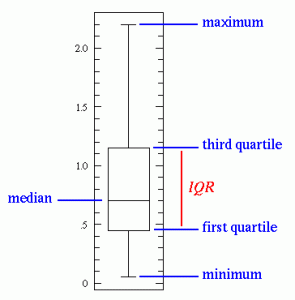
\includegraphics[width=6cm]{box-plot.png}
\end{figure}

\newpage
\section{Statistical Learning}
\subsection{What is Statistical Learning}
$n$ -- number of observations or training data.

$p$ -- number of features or parameters.

$x_{ij}$ -- the value of the $j$th predictor, or input, for observation $i$

$X = (x_1, \dots, x_p)$  -- input vector a.k.a features, predictors, independent variables.

$\epsilon$  -- error term, independent of $X$ and has mean zero.

$Y = f(X) + \epsilon$ -- a model a.k.a. output or dependent variable.

$y_i$ -- the response variable for the $i$th observation

In essence, statistical learning refers to a set of approaches for estimating $f$. 

\subsubsection{Why Estimate \texorpdfstring{$f$}{f}?}
There are two main reasons for estimating $f$: prediction and inference. 

\subsubsection*{Prediction}

We can predict $Y$ using $\hat Y = \hat f(X)$ where $\hat f$ represents an estimate of $f$ and $\hat Y$ represents the resulting prediction for $Y$. The accuracy of $\hat Y$ as a prediction for $Y$ depends on two quantities, the reducible error and the irreducible error. 

\textit{Reducible error} is the result of an inaccurate statistical learning technique.

\textit{Irreducible error} occurs because $Y$ is a function of $\epsilon$ which has variability that is dependent of $X$, so cannot be reduced via a statistical learning technique. Irreducible error may be larger than zero because of unmeasured variables or unmeasurable variation. The irreducible error will always provide an upper bound on the accuracy of our prediction for Y and is almost always unknown in practice.

\begin{equation}
    E[(Y - \hat f (x))^2 | X = x] = \underbrace{[f(x) - \hat f(x)]^2}_{\text{Reducible}} + \underbrace{Var(\epsilon)}_{\text{Irreducible}} 
\end{equation}

Note, $E(Y - \hat Y)^2 = E[(Y - \hat f (x))^2 | X = x] = E[f(X) + \epsilon - \hat f(X)]^2$ represents the average, or expected value, of the squared difference between the predicted and actual value of $Y$ and $Var(\epsilon)$ represents the variance associated with the error term  $\epsilon$. We square the values in order to ignore the resulting sign when finding averages.


\subsubsection*{Inference}
Often, we are interested in understanding how $Y$ changes as a function of $X_1,\dots,X_p$. That is, when we vary the value of a given feature, what should the result look like. Now $\hat f$ cannot be treated as a black box, because we need to know its exact form.

Common questions occurring in this setting include:
\begin{itemize}
    \item Which predictors are associated with the response?
    \item What is the relationship between the response and each predictor?
    \item Can the relationship between Y and each predictor be adequately summarized using a linear equation, or is the relationship more complicated? 
\end{itemize}

Depending on whether our ultimate goal is prediction, inference, or a combination of the two, different methods for estimating $f$ may be appropriate. Linear models allow for relatively simple and interpretable inference, but may not yield as accurate predictions as some other approaches. In contrast, some highly non-linear approaches can potentially provide quite accurate predictions for $Y$ at the expense of a less interpretable model, which makes inference more challenging.

\subsubsection{How Do We Estimate \texorpdfstring{$f$}{f}?}

Our training data or observations can be represented as ${(x_1, y_1),(x_2, y_2),...,(x_n, y_n)}$ where $x_i = (x_{i_1}, x_{i_2},...,x_{i_p})^T$ are vectors and $y_i$ are typically scalars.

Then, we want to find a function $\hat f$ such that $Y \approx \hat f(X)$ for any observation $(X, Y)$. Broadly speaking, most statistical learning methods for this task can be characterized as either \textit{parametric} or \textit{non-parametric}.

\subsubsection*{Parametric Methods}

This approach reduces the problem of estimating $f$ down to one of estimating a set of parameters.

\begin{enumerate}
    \item First, we make an assumption about the functional form, or shape, of $f$.
    
    \item After a model has been selected, we need a procedure that uses the training data to fit or train the model.
\end{enumerate}

For example, if we assume $f$ is linear, then $f(X) = \beta_0 + \beta_1X_1 + \beta_2X_2 + ... + \beta_p X_p$. To train the linear model, we need to estimate the parameters $\beta_0, \beta_1,..., \beta_p$, which is commonly done using (ordinary) least squares.


In general, fitting a more flexible model requires estimating a
greater number of parameters. These more complex models can lead to a phenomenon known as \textbf{overfitting} the data, which essentially means they follow the errors, or noise, too closely.

\subsubsection*{Non-parametric Methods}
Non-parametric methods do not make explicit assumptions about the functional form of $f$ and instead seek an estimate of $f$ that gets as close to the data points as possible while being reasonably smooth.

A very large number of observations (far more than is typically needed for a parametric approach) is required in order to obtain an accurate estimate for $f$. In order to fit a thin-plate spline, the data analyst must select a level of smoothness.

\subsubsection{The Trade-Off Between Prediction Accuracy and Model Interpretability}

\begin{figure}[H]
    \centering
    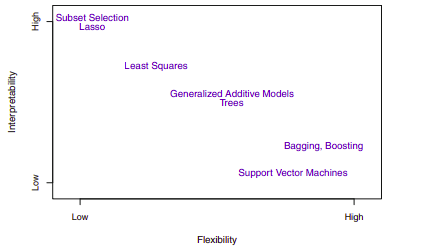
\includegraphics[width=11cm]{isl-figure-1.png}
\end{figure}


If we are mainly interested in inference, then restrictive models are much more interpretable.  In contrast, very flexible approaches, such as the splines and the boosting methods can lead to such complicated estimates of $f$ that it is difficult to understand how any individual predictor is associated with the response. 
Though there are clear advantages to using simple and relatively inflexible statistical learning methods when inference is the goal, the converse is not typically true. Instead we will often obtain more accurate predictions using a less flexible method. This phenomenon has to do with the potential for overfitting in highly flexible
methods.

\subsubsection{Supervised Versus Unsupervised Learning}
Most statistical learning problems fall into one of two categories: supervised or unsupervised.

In \textit{supervised learning}, for each observation of the predictor measurement(s) $x_i$, for $ i = 1,...,n$, there is an associated response measurement $y_i$. We wish to fit a model that relates the response to the predictors, with the aim of accurately predicting the response for future
observations (prediction) or better understanding the relationship between the response and the predictors (inference).

In contrast, \textit{unsupervised learning} describes the situation in which for every observation $i = 1,...,n$, we observe a vector of measurements $x_i$ but no associated response $y_i$. It is not possible to fit a linear regression model, since there is no response variable to predict.  One statistical learning tool that we may use in this setting is cluster analysis which aims to ascertain, on the basis of $x_1,..., x_n$, whether the observations fall into relatively distinct groups.

In a semi-supervised learning problem, we wish to use a statistical learning method that can incorporate the $m$ observations for which response measurements are available as well as the $n - m$ observations for which they are not. 

\subsubsection{Regression Versus Classification Problems}
Variables can be characterized as either quantitative (taking on numerical values) or qualitative/categorical. We tend to refer to problems with a quantitative response as regression problems, while those involving a qualitative response are often referred to as classification problems, but it's not always clear-cut and many problems can use either responses. Whether the predictors are qualitative or quantitative is generally considered less important provided that any qualitative predictors are properly coded before the analysis is
performed.

\subsection{Assessing Model Accuracy}

\subsubsection{Measuring the Quality of Fit}
In order to evaluate the performance of a statistical learning method on a given data set, we need to quantify the extent to which the predicted response value for a given observation is close to the true response value for that observation.

The most commonly-used measure is the \textit{mean squared error} (MSE), given by
\begin{equation}
    MSE = \frac{1}{n} \sum_{i=1}^n (y_i - \hat f(x_i))^2.
\end{equation}

The MSE computed using the training data that was used to fit the model can be referred to as the training
MSE. We want to choose the method that gives
the lowest test MSE, i.e. we want $\hat f(x_0)$ to be approximately equal to $y_0$, where $(x_0, y_0)$ is a previously unseen test observation not used to train the statistical learning method.

As model flexibility increases, training MSE will decrease, but the test MSE may not. When a given method yields a small training MSE but a large test MSE, we are said to be overfitting the data. This is a fundamental property of statistical learning that holds regardless of the particular data set at hand and regardless of the statistical method being used. When we overfit
the training data, the test MSE will be very large because the supposed patterns that the method found in the training data simply don’t exist in the test data. One important method for estimating test MSE using the training data is cross-validation, examined later. 

\subsubsection{The Bias-Variance Trade-Off}

The expected test MSE, for a given value $x_0$, can always be decomposed into the sum of three fundamental quantities: the variance of $\hat f(x_0)$, the squared bias of $\hat f(x_0)$ and the variance of the error terms. That is,

\begin{equation}
    E \Big (y_0 - \hat f(x_0) \Big )^2 = Var( \hat f(x_0)) + [Bias( \hat f(x_0))]^2 + Var(\epsilon).
\end{equation}

Here, $E \Big (y_0 - \hat f(x_0) \Big )^2$ defines the expected test MSE, computed by averaging the term over all possible values of $x_0$ in the test set. In order to minimize the expected test error, we need to select a statistical learning method that simultaneously achieves low variance and low bias. 

\textit{Variance} refers to the amount by which $\hat f$ would change if we estimated it using a different training data set. In general, more flexible statistical methods have higher variance. This is because changing any one of the data points may cause the estimate $\hat f$ to change considerably. A model with high variance does not generalize on the data which it hasn't seen before and is said to be overfitting.

\textit{Bias} refers to the error that is introduced by approximating a real-life problem, which may be extremely complicated, by a much simpler model. Generally, more flexible methods result in less bias. A model with high bias will be making overly strong assumptions about the training data and is said to be underfitting. 

\begin{figure}[h]
    \centering
    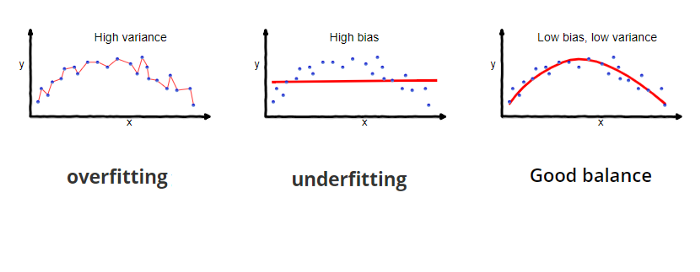
\includegraphics[width=13cm]{bias-variance-tradeoff.png}
\end{figure}
\vspace{-1cm} \begin{figure}[h]
    \centering
    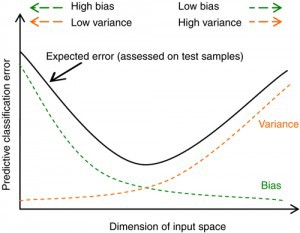
\includegraphics[width=7cm]{bias-variance-tuning.jpg}
\end{figure}
The relationship between bias, variance, and test set MSE is referred to as the \textit{bias-variance trade-off}. 

As a general rule, as we use more flexible methods, the variance will increase and the bias will decrease. The relative rate of change of these two quantities determines whether the test MSE increases or decreases. As we increase the flexibility of a class of methods, the bias tends to initially decrease faster than the variance increases. Consequently, the expected test MSE declines. However, at some point increasing flexibility has little impact on the bias but starts to significantly increase the variance. When this happens the test MSE increases. 
% (A model's assumption errors decrease faster than its ability to generalize to new observations)


\subsubsection{The Classification Setting}
Many of the previous concepts, including the bias-variance trade-off, transfer over to the classification setting with only some modifications due to the fact that $y_i$ is no longer numerical. Suppose that we seek to estimate $f$ on the basis of training observations $\{(x_1, y_1),...,(x_n, y_n)\}$, where now $y_1,...,y_n$ are qualitative.

The most common approach for quantifying the accuracy of our estimate $\hat f$ is the \textit{training error rate}, the proportion of mistakes that are made if we apply our estimated $\hat f$ to the training observations:

\begin{equation}
    \frac{1}{n} \sum_{i=1}^n I(y_i  \neq \hat y_i)
\end{equation}

Here $\hat y_i$ is the predicted class label for the $i$th observation using $\hat f$, and $I(y_i \neq \hat y_i)$ is an indicator variable that equals 1 if the $i$th observation was misclassified, i.e. $y_i \neq \hat y_i$, and equals zero if it was was classified correctly, i.e. $y_i = \hat y_i$.


The \textit{test error rate} associated with a set of test observations of the form $(x_0, y_0)$ is given by,
\begin{equation}
    Ave(I(y_0 \neq \hat y_0)),
\end{equation}
where $\hat y_0$ is the predicted class label. A good classifier minimizes the test error.

\subsubsection{The Bayes Classifier}
To minimize the test error rate, on average, we should simply assign a test observation with predictor vector $x_0$ to the class $j$ for which the conditional probability
\begin{equation}
    \Pr(Y = j|X = x_0)
\end{equation}
is largest. This very simple classifier is called the \textit{Bayes classifier}. In a two-class problem the classification will be class one if $Pr(Y = 1|X = x_0) > 0.5$, and class two otherwise. The line where the probability is exactly 0.5 is called the \textit{Bayes decision boundary}.

The Bayes classifier produces the lowest possible test error rate, called \textit{the Bayes error rate}, given by,
\begin{equation}
1 - E \Bigg( \max_j \Pr(Y = j|X) \Bigg ),
\end{equation}
where the expectation averages the probability over all possible values of $X$. The Bayes error rate is analogous to the irreducible error.

In theory we would always like to predict qualitative responses using the Bayes classifier. But for real data, we do not know the conditional distribution of $Y$ given $X$, and so computing the Bayes classifier is impossible. Therefore, the Bayes classifier serves as an unattainable gold standard against which to compare other methods.

\subsubsection{K-Nearest Neighbors}
Given a positive integer $K$ and a test observation $x_0$, the \textit{K-nearest neighbors} (KNN) classifier first identifies the $K$ points in the training data that are closest to $x_0$, represented by $\mathcal N_0$. It then estimates the conditional probability for class $j$ as the fraction of points in $\mathcal N_0$ whose response values equal $j$:

\begin{equation}
    \Pr(Y = j|X = x_0) = \frac{1}{K} \sum_{i \in \mathcal N_0} I(y_i = j).
\end{equation}

Finally, KNN applies Bayes rule and classifies the test observation $x_0$ to the class with the largest probability.

The choice of $K$ has a drastic effect on the KNN classifier obtained. As $K$ grows, the method becomes less flexible and produces a decision boundary that is close to linear. This corresponds to a low-variance but high-bias classifier. In
general, as we use more flexible classification methods, the training error rate will decline but the test error rate may not. In both the regression and classification settings, choosing the correct level of flexibility is critical to the success of any statistical learning method. The bias-variance tradeoff, and the resulting U-shape in the test error, can make this a difficult task. 

Nearest Neighbors can be good when the number of variables, $p$, is small, i.e. $p \leq 4$ and for a large number of sample points. It is one of many techniques called smoothers, like kernel and spline smoothing. Unfortunately this method is very poor when $p$ is large, since possible nearby neighbors tend to be far away in high dimensions. This is known as the \textit{curse of dimensionality}. We need to get a reasonable fraction of the $N$ values of $y_i$ to average in order to bring the variance of our model down. However, as we increase the dimensions, the radius we need to search increases and we lose the efficacy of estimating using local averages.

\newpage
\section{Linear Regression}
\textit{Linear regression} is a very simple approach for supervised learning and is a useful tool for predicting a quantitative response.

\subsection{Simple Linear Regression}

Simple linear regression  is a very straightforward approach for predicting a quantitative response $Y$ on the basis of a single predictor variable $X$. It assumes that there is approximately a linear relationship between $X$ and $Y$. We will sometimes describe this by saying that we are regressing $Y$ on $X$.
\begin{equation}
    Y \approx \beta_0 + \beta_1 X
\end{equation}
$\beta_0$ and $\beta_1$ are two unknown constants that represent the intercept and slope terms in the linear model and are known as its coefficients or parameters. We may use our training data to produce estimates $\hat \beta_0$ and $\hat \beta_1$ for prediction,
\begin{equation}
    \hat y  \approx \hat \beta_0 + \hat \beta_1 x,
\end{equation}
where $\hat y$ indicates a prediction of $Y$ on the basis of $X = x$.


\subsubsection{Estimating the Coefficients}
Let $(x_1, y_1), (x_2, y_2),..., (x_n, y_n)$ represent $n$ observation pairs, each of which consists of a measurement of $X$ and a measurement of $Y$. We want to find an intercept $\hat \beta_0 $ and a slope $\hat \beta_1$ such that the resulting line is as close as possible to the $n$ data points. The most common definition of closeness involves minimizing the least squares criterion.

Let $\hat y_i = \hat \beta_0 + \hat \beta_1 x_i$ be the prediction for $Y$ based on the $i$th value of $X$. Then $e_i = y_i - \hat y_i$ represents the $i$th residual -- this is the difference between $i$th observed response and its prediction. 

We define the \textit{residual sum of squares (RSS)} as,
\begin{align}\label{eq:RSS}
\begin{split}
     RSS &= e_1^2 + e_2^2 + \dots + e_n^2\\
     &=  (y_1 - \hat \beta_0 - \hat \beta_1 x_1)^2 + \cdots + 
     (y_n - \hat \beta_0 - \hat \beta_1 x_n)^2
\end{split}
\end{align}

The least squares approach chooses $\hat \beta_0 $ and $\hat \beta_1$ to minimize the RSS.

Let $ \bar y \equiv \frac{1}{n} \sum^n_{i=1} y_i$ and $\bar x \equiv \frac{1}{n} \sum_{i=1}^n x_i$ be the sample means. Then the the \textit{least squares coefficient estimates} are given by,

\begin{align*}
    \hat \beta_0 &= \frac{\sum_{i=1}^n (x_i - \bar x) (y_i - \bar y)}{\sum_{i=1}^n (x_i - \bar x)^2}, \\ 
    \hat \beta_1 &= \bar y - \hat \beta_1 \bar x.
\end{align*}

 
\subsubsection{Assessing the Accuracy of the Coefficient Estimates}

If $f$ is to be approximated by a linear function, then we can write this relationship as a \textit{population regression line},
\begin{align*}
 Y &= f(X) +  \epsilon \\
 Y  &= \beta_0 +  \beta_1 X + \epsilon
\end{align*}
Where $\beta_0$ is the intercept, i.e. the expected value of $Y$ when $X = 0$, $\beta_1$ is the slope, i.e.  the average increase in $Y$ in a unit of increase of $X$, and $\epsilon$ is a catch-all error term.
 
The \textit{least squares line} can always be computed using the coefficient estimates, however, the population regression line is unobserved. Fundamentally, the concept of these two lines is a natural extension of the standard statistical approach of using information from a sample to estimate characteristics of an unmeasured large population.
 
The analogy between linear regression and estimation of the mean of a
random variable is an apt one based on the concept of bias. if we could average a huge number of estimates $\hat \mu$ of the true population mean $\mu$ obtained from a huge number of sets of observations, then this average would exactly equal $\mu$. Thus it is an unbiased estimator, i.e. it does not systematically over- or under-estimate the true parameter. 

To determine the accuracy of a sample mean $\hat \mu$ as an estimate of $\mu$, we can find the \textit{standard error}, which roughly tells us the average amount that this estimate differs from the actual value of $\mu$,
\begin{equation}
    \text{Var} (\hat \mu) = \text{SE} (\hat \mu ) ^2 = \frac{\sigma^2}{n},
\end{equation}
where $\sigma$ is the standard deviation of each of the realizations $y_i$ of $Y$.

To compute the standard errors associated with $\hat \beta_0$ and $\hat \beta_1$,

\begin{align*}
    \text{SE} ( \hat \beta_0 )^2 &= \sigma^2 \Bigg (  \frac{\bar x^2}{(x_i - \bar x)^2}  \Bigg )\\ 
    \text{SE} ( \hat \beta_1 )^2 &= \frac{\sigma^2}{\sum_{i=1}^n (x_i - \bar x)^2} 
\end{align*}

where $\sigma^2 = \text{Var}(\epsilon)$. In general, $\sigma^2$ is not known, but can be estimated from the data. The estimate of $\sigma$ is known as the \textit{residual standard error}, and is given by the formula,
\begin{equation}\label{eq:RSE-1}
    RSE = \sqrt{RSS/(n - 2)}
\end{equation}

Standard errors can be used to compute \textit{confidence intervals}. For example, a  95\% confidence interval is defined as a range of values such that with  95\% probability, the range will contain the true unknown value of the parameter.For linear regression the confidence interval of the coefficients is given by,
\begin{align*}
    \hat \beta_1 &\pm 2 \cdot \text{SE}(\hat \beta_1)  \\
    \hat \beta_0 &\pm 2 \cdot \text{SE}(\hat \beta_0).
\end{align*}
Standard errors can also be used to perform hypothesis tests on the coefficients. The null hypotheses --  $H_0$ : There is no relationship between $X$ and $Y$, i.e. $\beta_1 = 0$. The alternative hypothesis -- $H_a$ : There is some relationship between $X$ and $Y$, i.e. $\beta_1 \neq 0$. 

Notice that setting $\beta_1 = 0$ removes the $X$ term in $Y = \beta_0 + \beta_1 X + \epsilon$ and $X$ is not associated with $Y$. So if $\hat \beta_1$ is sufficiently far from zero and $\text{SE}(\hat \beta_1)$ is small, then our estimates of the parameter our accurate and give strong evidence that the null hypotheses is true. if $SE(\hat\beta_1)$ is large, then $SE(\hat\beta_1)$ must be large in absolute value in order for us to reject the null hypothesis.

In practice, we compute the \textit{t-statistic}, given by,
\begin{equation}
    t = \frac{\hat \beta_1 - 0}{\text{SE}(\hat \beta_1)}
\end{equation}
which measures the number of standard deviations that $\hat \beta_1$ is away from 0. If there is no relationship between $X$ and $Y$, the t-statistics will have a distribution with $n - 2$ degrees of freedom. 

The \textit{p-value} corresponds to the probability of observing any number equal to $|t|$ or larger in absolute value, assuming $\beta_1= 0$. A small p-value indicates that it is unlikely to observe such a substantial association between the predictor and the response due to chance, in the absence of any real association, so we can infer that there is an association between the predictor and the response. Then, we can reject the null hypothesis and may declare a relationship between $X$ and $Y$ if the p-value is small enough.

Simply put, a p-value is the probability that random chance generated the data, or (plus) it was the result of another event that is of equal or rarer probability. The traditional threshold for determining significance of a p-value is $< 0.05$.

\subsubsection{Assessing the Accuracy of the Model}
Given the alternative hypothesis holds, we likely want to quantify the extent to which the model fits the data. A linear regression fit is typically assessed using two related quantities: the residual standard error (RSE) and the $R^2$ statistic.

\subsubsection*{Residual Error}
The RSE is an estimate of the standard deviation of the irreducible error term $\epsilon$. Roughly speaking, it is the average amount that the response
will deviate from the true regression line and is considered a measure of the lack of fit of the model to the data. 

Recall, RSS is the residual sum of squares \eqref{eq:RSS} and the RSE was previously used to estimate $\sigma$ \eqref{eq:RSE-1}. Then, the RSE can be written as,
\begin{equation}
    RSE = \sqrt{\frac{1}{(n-2)} \text{RSS} } 
    = \sqrt{\frac{1}{(n-2)} \sum_{i=1}^n (y_i - \hat y_i)^2 }.
\end{equation}

\subsubsection*{\texorpdfstring{$R^2$}{R-Squared} Statistic} 
The $R^2$ statistic provides an alternative measure of fit in terms of the proportion of explained variance, i.e. not residual, and so it always takes on a value between 0 and 1. Moreover, it is independent of the scale of $Y$, unlike the RSE. The $R^2$ statistic is a measure of the linear relationship between $X$ and $Y$.

Let $\text{TSS} = (y_i - \hat y)^2$ be the \textit{total sum of squares} and RSS be the residual sum of squares \eqref{eq:RSS}. Then $R^2$ is given by,
\begin{equation}
    R^2 =  \frac{\text{TSS} - \text{RSS}}{\text{TSS}} = 1 - \frac{RSS}{TSS}
\end{equation}

TSS can be thought of as the amount of variability inherent in the response before the regression is performed while RSS measures the amount of variability that is left unexplained after performing the regression. TSS - RSS measures the amount of variability in the response that is explained (or
removed) by performing the regression, and $R^2$ measures the proportion of variability in $Y$ that can be explained using $X$.

An $R^2$ statistic that is close to 1 indicates that a large proportion of the variability in the response has been explained by the regression, while the converse holds for a value close to 0. The $R^2$ statistic is similar to correlation, but holds for a between a larger number of variables.

\subsection{Multiple Linear Regression}
We can handle multiple predictors by giving each predictor a separate slope coefficient in a single model. In general, suppose that we have $p$ distinct predictors. Then the multiple linear regression model takes the form,
\begin{equation}
    Y = \beta_0 + \beta_1 X_1 + \beta_2 X_2 + \dots + \beta_p X_p + \epsilon,
\end{equation}
where $X_j$ represents the $j$th predictor and $\beta_j$ quantifies the association between that variable and the response, namely the average effect on $Y$ of a one unit increase in $X_j$  while holding all other predictors fixed.

\subsubsection{Estimating the Regression Coefficients}

Given estimates $\hat \beta_0, \hat \beta_1,..., \hat \beta_p$, we can make predictions using the formula,
\begin{equation}
     \hat y= \hat \beta_0, \hat \beta_1 x_1,..., \hat \beta_p x_p.
\end{equation}
Again, we choose $\beta_0, \beta_1,...,\beta_p$ to minimize the residual sum of squared,
\begin{align*} \label{eq:RSS-sum}
    RSS &= \sum_{i=1}^{n} (y_i - \hat y_i)^2 \\
    &=  \sum_{i=1}^{n}(y_i - \hat \beta_0 - \hat \beta_1 x_1,..., \hat \beta_p x_p)^2 \\
    &= \sum_{i=1}^n \Bigg ( y_i - \beta_0 - \sum_{j=1}^p \beta_j x_{ij} \Bigg)^2
\end{align*}
The values $\hat \beta_0, \hat \beta_1 x_1,..., \hat \beta_p x_p$ that minimize the above equation are the multiple least squares regression coefficient estimates. These values are most easily represented using matrix algebra and will be revisited later.

\subsubsection{Some Important Questions}
\begin{enumerate}
    \item Is at least one of the predictors $X_1, X_2,...,X_p$ useful in predicting the response?
    \item Do all the predictors help to explain $Y$, or is only a subset of the predictors useful?
    \item How well does the model fit the data? 
    \item Given a set of predictor values, what response value should we predict, and how accurate is our prediction?
\end{enumerate}

\subsubsection*{Is There a Relationship Between the Response and Predictors?}
In the multiple regression setting with $p$ predictors, we need to ask whether all of the regression coefficients are zero. The null hypothesis becomes,
\begin{equation}
    H_0 : \beta_1 = \beta_2 = \dots = \beta_p = 0.
\end{equation}

This hypothesis test is performed by computing the \textit{F-statistic}.
\begin{equation}
    F = \frac{(\text{TSS} - \text{RSS})/p }{\text{RSS}/ (n-p-1)}
\end{equation}

When there is no relationship between the response and predictors, one would expect the F-statistic to take on a value close to 1. On the other hand, if $H_a$ is true (i.e. at least one $\beta_j$ is non-zero.), then $E{(\text{TSS} - \text{RSS})/p} > \sigma^2$, so we expect $F$ to be greater than $1$.

The approach of using an F-statistic to test for any association between the predictors and the response works when $p$ is relatively small, and certainly small compared to $n$. However, sometimes we have a very large number of variables. If $p>n$ then there are more coefficients $\beta_j$ to estimate than observations from which to estimate them. In this case we cannot even fit the multiple linear regression model using least squares, so the F-statistic cannot be used. Approaches like \textit{forward selection} can be used instead.

\subsubsection{Deciding on Important Variables}
The first step in a multiple regression analysis is to compute the F-statistic and to examine the associated p-value. If we conclude on the basis of the p-value that at least one of the predictors is related to the response, then it is natural to wonder which are the relevant ones. The task of determining which predictors are associated with the response, in order to fit a single model involving only those predictors, is referred to as \textit{variable selection}, discussed more in detail in chapter 6.

There are a total of $2^p$ models that contain subsets of $p$ variables. In general, we cannot consider all $2^p$ models, and instead we need an automated and efficient approach to choose a smaller set of models to consider. There
are three classical approaches for this task:
\begin{enumerate}
    \item \textit{Forward selection} -- We begin with the null model, i.e. a model that contains an intercept (i.e $\beta_0$) but no predictors. We then fit $p$ simple linear regressions and add to the null model the variable that results in the lowest RSS. We then add to that model the variable that results in the lowest RSS for the new two-variable model. This approach is continued until some stopping rule is satisfied.
    
    \item \textit{Backward selection} -- We start with all variables in the model, and remove the variable with the largest p-value—that is, the variable  that is the least statistically significant. The new ($p - 1$)-variable model is fit, and the variable with the largest p-value is removed. This procedure continues until a stopping rule is reached, i.e. when  all remaining variables have a p-value below some threshold.
    
    \item \textit{Mixed selection} -- This is a combination of forward and backward selection. We start with no variables in the model, and as with forward selection, we add the variable that provides the best fit. Since the p-values for variables can become larger as new predictors are added to the model, if at any point the p-value for one of the variables in the model rises above a certain threshold, then we remove that variable from the model. We continue to perform these forward and backward steps until all variables in the model have a sufficiently low p-value.
\end{enumerate}

Backward selection cannot be used if $p>n$, while forward selection can
always be used. Forward selection is a greedy approach, and might include
variables early that later become redundant. Mixed selection can remedy
this.

\subsubsection*{Model Fit}
In multiple linear regression, $R^2 =  Cor(Y, \hat Y)^2$,  the square of the correlation between the response and the fitted linear model. $R^2$ will always increase when more variables are added to the model, even if they are only weakly associated with the response.  This is due to the fact that adding another variable to the least squares equations must allow us to fit the training data more accurately, so the $R^2$ statistic, which is also computed on the training data, must increase.

\subsubsection*{Predictions}
After fitting a regression model, there are three sorts of uncertainty associated with a prediction.
\begin{enumerate}
    \item There will be some inaccuracy in the coefficient estimates related to the reducible error of using the least squares plane. We can compute a \textit{confidence interval} in order to determine how close $\hat Y$ will be to $f(X)$.
    \item There is potentially an additional source of reducible error, called \textit{model bias}, from using a linear model to represent complex non-linear data.
    \item There will be some amount of irreducible or random error in the model.  \textit{Prediction intervals} are used to incorporate both the error in the estimate for $f(X)$ (the reducible error) as is done in a confidence interval, as well as the uncertainty as to how much an individual point will differ from the population regression plane (the irreducible error). 
\end{enumerate}


\subsection{Other Considerations in the Regression Model}
\subsubsection{Qualitative Predictors}
\subsubsection*{Predictors with Only Two Levels}
If a qualitative predictor (also known as a factor) only has two levels, or possible values, then incorporating it into a regression model is very simple. We simply create an indicator or dummy variable that takes on two possible numerical values, i.e. (0 or 1) and use this variable as a predictor in the regression equation.

\subsubsection*{Qualitative Predictors with More than Two Levels}
In this situation, we can create additional dummy variables. There will always be one fewer dummy variable than the number of levels. The level with no dummy variable is known as the \textit{baseline}.

\subsubsection{Extensions of the Linear Model}
Two of the most impactful assumptions in the standard linear regression model state that the relationship between the predictors and response are additive and linear. The \textit{additive} assumption means that the effect of changes in a predictor $X_j$ on the response Y is independent of the values of the other predictors. The \textit{linear} assumption states that the change in the response $Y$ due to a one-unit change in $X_j$ is constant, regardless of the value of $X_j$.

\subsubsection*{Removing the Additive Assumption}
One way of extending this model to allow for interaction effects is to include a third predictor, called an \textit{interaction term} $\Tilde \beta_1$, which is constructed by computing the product of X1 and X2.
\begin{align*}
    Y &= \beta_0 + \beta_1 X_ 1 + \beta_2 X_2 + \beta_3 X_1 X_2 + \epsilon \\
    &= \beta_0 + (\beta_1 + \beta_3 X_2)X_1 + \beta_2 X_2 + \epsilon \\
    &= \beta_0 + \Tilde \beta_1 X_1 + \beta_2 X_2 + \epsilon
\end{align*}
Then, adjusting $X_2$ will change the impact of $X_1$ on $Y$.

The \textit{hierarchical principle} states that if we include an interaction in a model, we should also include the main effects, even if the p-values associated with their coefficients are not significant.
 
\subsubsection*{Non-linear Relationships}
In some cases, the true relationship between the response and the predictors may be nonlinear. A simple way to directly extend the linear model to accommodate non-linear relationships is to use \textit{polynomial regression}, in which we include polynomial functions of the predictors in the regression model.

\subsubsection{Potential Problems and Troubleshooting}
\begin{enumerate}
    \item Non-linearity of the response-predictor relationships.
    
        Residual plots are useful graphical tool for identifying non-linearity. If there is a strong pattern in the  plot of the residuals, $e_i = y_i - \hat y_i$, versus the predictor $x_i$, there may be a problem with some aspect of the linear model.
    
    \item Correlation of error terms.
    
         In general, the assumption of uncorrelated errors is extremely important for linear regression as well as for other statistical methods.
        
        If there is correlation among the error terms, then the estimated standard errors will tend to underestimate the true standard errors, confidence and prediction intervals will be narrower than they should be, and p-values associated with the model will be lower than they should be.  Such correlations frequently occur in the context of time series data.
        
        We can plot the residuals from our model as a function of time and if the errors are uncorrelated, then there should be no discernible pattern. Otherwise we may find that \textit{tracking} exists, i.e. adjacent residuals often have similar values.
    
    \item Non-constant variance of error terms.
        
        An important assumption is that error terms have constant variance, i.e. $ \text{Var}(\epsilon_i) = \sigma^2$.  One can identify non-constant variance, a.k.a. \textit{heteroscedasticity}, from the presence of a funnel shape in the residual plot.
        
        A simple remedy may be to fit our model by \textit{weighted least squares}, with weights proportional to the inverse weighted variances.
    
    \item Outliers.
    
    A point for which $y_i$ is far from the value predicted by the model can occur for many reasons, possibly as a result  of incorrect recording of an observation.
    It is typical for an outlier that does not have an unusual predictor value to have little effect on the least squares fit, but may have an effect on the RSE, used to compute all confidence intervals or p-values, as well as $R^2$. 
    
    Residual plots can be used to identify outliers, but in practice, it can be difficult to decide how large a residual needs to be before we consider the point to be an outlier. Instead, we can plot the \textit{studentized residuals}, computed by dividing each residual $e_i$ by its estimated standard error. Observations whose studentized residuals are greater than 3 in absolute value are possible outliers and can be removed or examined to determine a deficiency with the model, such as a missing predictor.
    
    \item High-leverage points.
    
    In contrast to outliers, observations with \textit{high leverage} have an unusual value for $x_i$. Removing a high leverage observation has a much more substantial impact on the least squares line than removing the outlier.
    
    To quantify an observation’s leverage, we compute the \textit{leverage statistic}. The leverage statistic $h_i$ is always between $1/n$ and $1$, and the average leverage for all the observations is always equal to $(p + 1)/n$. For a simple linear regression,
    \begin{equation}\label{eq:leverage}
        h_i =  \frac{1}{n} \frac{(x_i - \bar x)^2}{\sum_{i' = 1}^n (x_i - \bar x)^2}
    \end{equation}
    
    \item Collinearity.
    
    \textit{Collinearity} refers to the situation in which two or more predictor variables are closely related to one another. In the regression context, it can be difficult to separate out the individual effects of collinear variables on the response and reduces the accuracy of the estimates of the regression coefficients. This causes the standard error for $\hat \beta_j$ to grow and the t-statistic to decline which in turn means the power of the hypothesis test - the probability of correctly detecting a non-zero coefficient - is reduced by collinearity.
    
    A simple way to detect collinearity is to look at the correlation matrix of the predictors, though this may not always work. In particular, it is possible for collinearity to exist between three or more variables in what's called \textit{multicollinearity}. In this situation it's better to compute the \textit{variance inflation factor} (VIF), the ratio of the variance of $\hat \beta_j$ when fitting the full model divided by the variance of $\hat \beta_j$ if fit on its own. A VIF value of 1 indicates the complete absence of collinearity, a VIF value that exceeds 5 or 10 indicates a problematic amount of collinearity.
    
    \begin{equation}
        VIF(\hat \beta_j ) = \frac{1}{1-R^2_{X_j|X_{-j}}}
    \end{equation}
    where $R^2_{X_j|X_{-j}}$ is the $R^2$ from a regression of $X_j$ onto all of the other predictors.
    
    To mitigate collinerarity, we may drop one of the problematic variables from the regression, which will also reduce redundancy. Alternatively, we may combine the collinear variables together into a single predictor.
    
\subsection{Comparison of Linear Regression with K-Nearest Neighbors}
Linear regression is an example of a parametric approach and has many advantages: they are often easy to fit, the coefficients have simple interpretations, and tests of statistical significance can be easily performed. But parametric methods do have a disadvantage: by construction, they make strong assumptions about the form of $f(X)$. 

In contrast, non-parametric methods do not explicitly assume a parametric form for $f(X)$, and thereby provide an alternative and more flexible approach for performing regression. 

One of the simplest and best-known non-parametric methods is \textit{K-nearest neighbors regression} (KNN regression), which is closely related to the KNN classifier.

Given a value for $K$ and a prediction point $x_0$, KNN regression first identifies the $K$ training observations that are closest to $x_0$, represented by $\mathcal N_0$. It then estimates $f(x_0)$ using the average of all the training responses in $\mathcal N_0$. In general, the optimal value for K will depend on the bias-variance tradeoff.

\begin{equation}
    \hat f (x_0) = \frac{1}{K} \sum_{x_i \in \mathcal N_0} y_i.
\end{equation}

The parametric approach will outperform the nonparametric approach if the parametric form that has been selected is close to the true form of $f$. Even when the true relationship is highly non-linear, KNN may still provide inferior results to linear regression. A decrease in performance as the dimension increases is a common problem for KNN, and results from the fact that in higher dimensions there is effectively a reduction in sample size. As a general rule, parametric methods will tend to outperform non-parametric approaches when there is a small number of observations per predictor.

\newpage
\section{Classification}

\subsection{An Overview of Classification}
The linear regression model assumes that the response variable $Y$ is quantitative. But in many situations, the response variable is instead qualitative. Though just as in the regression setting, in the classification setting we have a set of training observations $(x_1, y_1),\dots,(x_n, y_n)$.

\subsection{Why Not Linear Regression}
Linear regression is not appropriate in the case of a qualitative response since codings of qualtative states into numeric values may produce unwarranted implicit relations with each of the codings depending on their orderings. This can produce fundamentally different linear models that would ultimately lead to different sets of predictions on test observations.

For a binary (two level) qualitative response we could potentially use the dummy variable approach to code the response and could then fit a linear regression to it. However, if we use linear regression, some of our estimates might beoutside the [0, 1] interval, making them hard to interpret as probabilities. Nevertheless, the predictions provide an ordering and can be interpreted as crude probability estimates. It turns out that the classifications that we get if we use linear regression to predict a binary response will be the same as for the linear discriminant analysis (LDA) procedure discussed later.

\subsection{Logistic Regression}
\subsubsection{The Logistic Model}
Any time a straight line is fit to a binary response that is coded as $0$ or $1$, in principle we can always predict $p(X) < 0$ for some values of $X$ and $p(X) > 1$ for others (unless the range of $X$ is limited). Instead, we must model $p(X)$ using a function that gives outputs between $0$ and $1$ for all values of $X$. Many functions meet this description. In logistic regression, we use the logistic function,
\begin{equation}
    p(X) = \frac{e^{\beta_0 + \beta_1 X}}{1 + e^{\beta_0 + \beta_1 X}}
\end{equation}
To fit the model, we use a method called \textit{maximum likelihood}, discussed in the next section. The logistic function will always produce an S-shaped curve, and so regardless of the value of $X$, we will obtain a sensible prediction. After a bit of manipulation, we find that,
\begin{equation}
    \frac{p(X)}{1-p(X)} = e^{\beta_0+\beta_1 X}
\end{equation}
The quantity on the left-hand side is called the \textit{odds} and can take on any value between 0 and $\infty$, indicating very low and high probabilities. Odds are traditionally used instead of probabilities in horse-racing, since they relate more naturally to the correct betting strategy.

By taking the logarithm of both sides,
\begin{equation}
    \log \Bigg ( \frac{p(X)}{1-p(X)} \Bigg ) = \beta_0+\beta_1 X
\end{equation}

The left-hand side is called the \textit{log-odds} or \textit{logit}. We see that the logistic regression model has a logit that is linear in $X$.

Recall that in a linear regression model, $\beta_1$ gives the average change in $Y$ associated with a one-unit increase in $X$. In contrast, in a logistic regression model, increasing $X$ by one unit changes the log odds by $\beta_1$, or equivalently it multiplies the odds by $e^{\beta_1}$. The amount that $p(X)$ changes due to a one-unit change in $X$ will depend on the current value of $X$, though if $\beta_1$ is positive then increasing $X$ will be associated with increasing $p(X)$,
and if $\beta_1$ is negative then increasing $X$ will be associated with decreasing $p(X)$.

\subsubsection{Estimating the Regression Coefficients}
The coefficients $\beta_0$ and $\beta_1$  are unknown, and must be estimated based on the available training data. \textit{Maximum likelihood} is used to fit a logistic regression model instead of least squares. The estimates $\hat \beta_0$ and $\hat\beta_1$ are chosen to maximize what's called the \textit{likelihood function}:
\begin{equation}
    l(\beta_0,\beta_1) = \prod_{i:y_i = 1} p(x_i) \prod_{i':y_{i' = 1}} (1-p(x_{i'}))  
\end{equation}
Maximum likelihood is a very general approach that is used to fit many non-linear models. In the linear regression setting, the least squares approach is in fact a special case of maximum likelihood.

Many aspects of the logistic regression are similar to the linear regression output. For example, we can measure the accuracy of the coefficient estimates by computing their standard errors. The \textit{ $z$-statistic} plays the same role as the $t$-statistic in the linear regression output. the $z$-statistic associated with $\beta_1$ is equal to $\hat \beta_1/SE(\hat\beta_1)$, and so a large (absolute) value of the $z$-statistic indicates evidence against the null hypothesis $H_0 : \beta_1 = 0$. This null hypothesis implies that $p(X) = \frac{e^{\beta_0}}{1+e^{\beta_0}}$.

\subsubsection{Making Predictions}
Once the coefficients have been estimated, it is a simple matter to compute
the probability. We can then use qualitative predictors with the logistic regression model to fit the model by using the dummy variable approach mentioned previously, i.e. the variable takes on a value of 1 or 0. If the coefficient associated with the dummy variable is positive and the associated p-value is statistically significant, this will validate that there is a higher probability associated with the encoded qualitative state.

\subsubsection{Multiple Logistic Regression}
By analogy with the extension from simple to multiple linear
regression, we can generalize the logistic model as follows,
\begin{equation}
    \log \Bigg ( \frac{p(X)}{1-p(X)} \Bigg ) = \beta_0+\beta_1 X_1 + \dots + \beta_pX_p,
\end{equation}
where $X = (X_1,...,X_p)$ are $p$ predictors. This can be rewritten as,
\begin{equation}
    p(X) = \frac{e^{\beta_0+\beta_1 X_1 + \dots + \beta_pX_p}}{1+e^{\beta_0+\beta_1 X_1 + \dots + \beta_pX_p}}
\end{equation}
Just as before, we use the maximum likelihood method to estimate $\beta_0, \beta_1,\dots,\beta_p$.

\subsubsection{Logistic Regression for \texorpdfstring{$>2$}{greater than 2} Response Classes}

Suppose we want to classify a response variable that has more than two classes. The two-class logistic regression models discussed in the previous sections have multiple-class extensions, but in practice they tend not to be used all that often. Instead, a more popular multiple-class classification method known as, \textit{discriminant analysis}, is used.

\subsection{Linear Discriminant Analysis}
Logistic regression involves directly modeling $Pr(Y = k|X = x)$ using the logistic function to model the conditional distribution of the response $Y$, given the predictor(s) $X$. In an alternative and less direct approach to estimating these probabilities, we model the distribution of the predictors $X$ separately in each of the response classes (i.e. given $Y$), and then use Bayes’ theorem \eqref{eq:bayes} to flip these around into estimates for $Pr(Y = k|X = x)$. When these distributions are assumed to be normal the model is very similar in form to logistic regression.

Linear discriminant analysis is a useful alternative to logistic regression because:
\begin{itemize}
    \item When the classes are well-separated, the parameter estimates for the logistic regression model are surprisingly unstable. Linear discriminant analysis does not suffer from this problem.
    \item If $n$ is small and the distribution of the predictors $X$ is approximately normal in each of the classes, the linear discriminant model is again more stable than the logistic regression model.
    \item As mentioned, linear discriminant analysis is popular when we have more than two response classes.
\end{itemize}

\subsubsection{Using Bayes’ Theorem for Classification}
Suppose the qualitative response variable $Y$ can take on $K>2$ possible distinct and unordered values. Let $\pi_k$ represent the overall or \textit{prior} probability that a randomly chosen observation comes from the $k$th class or category of the response variable $Y$.

If $X$ is a discrete random variable, Let $f_k(X) = \Pr(X = x|Y = k)$ denote
the \textit{density function} of $X$ for an observation that comes from the $k$th class. The densiity function is relatively large if there is a high probability that an observation in the kth class has $X \approx x$ and small otherwise. Then \textit{Bayes’ theorem} states that,

\begin{equation}\label{eq:bayes}
    \Pr(Y = k| X = x) = \frac{\pi_k f_k (x) }{ \sum_{l=1}^{K} \pi_l f_l(x)}.
\end{equation}

Recall, $p_k(X) = \Pr(Y = k|X)$. We refer to $p_k(x)$ as the \textit{posterior} probability that an observation belongs to the kth class, given the predictor value for that observation, i.e. $X = x$. This suggests that instead of directly computing $p_k(X)$ as was done in previous methods, we can plug in estimates of $\pi_k$ and $f_k(X)$ into the above formula. Estimating the pripor probabilities $\pi_k$ is easy if we have a random sample of $Y$s from the population: we simply compute the fraction of the training observations that belong to the $k$th class. However, estimating $f_k(X)$ tends to be more challenging, unless we assume some simple forms for these densities. 

Recall the Bayes classifier, which classifies an observation to the class for which $p_k(X)$ is largest, has the lowest possible error rate out of all classifiers. Therefore, if we can find a way to estimate $f_k(X)$, then we can develop a classifier that approximates the Bayes classifier. 

\subsubsection{Linear Discriminant Analysis for \texorpdfstring{$p=1$}{p = 1}}
Assume that we only have one predictor, i.e. $p=1$. To obtain an estimate for $f_k(x)$ to plug into the Linear Discriminant Analysis formula we will first make some assumptions about its form.

Suppose we assume that $f_k(x)$ is \textit{normal} or \textit{Gaussian}. In the one-dimensional setting, the normal density takes the form,
\begin{equation}\label{eq:gaussian}
    f_k(x) = \frac{1}{\sqrt{2\pi} \sigma_k} \exp \Bigg ( -\frac{1}{2\sigma^2_k} (x-\mu_k)^2 \Bigg) 
\end{equation}

where $\mu_k$ and  $\sigma^2_k$ are the mean and variance parameters for the $k$th class. We may assume there is a shared variance term across all $K$ classes, i.e. $\sigma^2_1 = \dots = \sigma^2_K$, which for simplicity we can denote by $\sigma^2$. 

We can then plug this into Bayes' theorem \eqref{eq:bayes},
\begin{equation}
    p_k(x) = \frac{
        \pi_k \frac{1}{\sqrt(2\pi) \sigma_k} \exp \Big ( -\frac{1}{2\sigma^2_k} (x-\mu_k)^2 \Big)  
    }{
         \sum_{l=1}^{K} \pi_l \frac{1}{\sqrt(2\pi) \sigma_k} \exp \Big ( -\frac{1}{2\sigma^2_k} (x-\mu_k)^2 \Big) 
    }.  
\end{equation}

Taking the log and rearranging the terms shows us that assigning an observation in a Bayes' classifier is equivalent to assigning the observation to the class for which the following equation is the largest:

\begin{equation}\label{eq:lda-delta}
    \delta_k(x) = x \cdot \frac{\mu_k}{\sigma^2} -\frac{\mu_k^2}{2\sigma^2} + \log(\pi_k)
\end{equation}

In practice, even if we are quite certain of our assumption that $X$ is drawn from a Gaussian distribution within each class, we still have to estimate the parameters $\mu_1,...,\mu_K$, $\pi_1,..., \pi_K$, and $\sigma^2$. The \textit{linear discriminant analysis} (LDA) method approximates the Bayes classifier by plugging estimates for $\pi_k, \mu_k$, and $\sigma^2$ into the above \eqref{eq:lda-delta}.  In particular, the following estimates are used:
\begin{align}
\begin{split}
    \hat \mu &=  \frac{1}{n^k} \sum_{i:y_i = k} x_i \\
    \hat \sigma^2 &= \frac{1}{n-K} \sum_{k=1}^K \sum_{i:y_i = k} (x_i - \hat \mu_k)^2 
\end{split}
\end{align}
where $n$ is the total number of training observations and $n_k$ is the number
of training observations in the $k$th class. The estimate for $\mu_k$ is simply the average of all the training observations from the $k$th class, while $\hat\sigma^2$ can be seen as a weighted average of the sample variances for each of the $K$ classes.

Sometimes we have knowledge of the class membership probabilities $\pi_1,...,\pi_K$, otherwise LDA estimates $\pi_k$ using the proportion of the training observations that belong to the $k$th class, i.e,
\begin{equation}
    \hat \pi_k = \frac{n_k}{n}.
\end{equation}

When plugging the above estimates into $\delta_k$ \eqref{eq:lda-delta}, they become the \textit{discriminant functions}, $\hat \delta_k(x)$. The word linear in the classifier’s name stems from the fact that the discriminant functions $\hat \delta_k$ are linear functions of $x$. Again, we assign an observation $X = x$ to the class for which $\hat \delta_k$ is largest:
\begin{equation}
    \hat \delta_k(x) = x \cdot \frac{\hat \mu_k}{\hat \sigma^2} -\frac{\hat \mu_k^2}{2 \hat \sigma^2} + \log(\hat \pi_k).
\end{equation}

To reiterate, the LDA classifier results from assuming that the observations within each class come from a normal distribution with a class-specific mean vector and a common variance $\sigma^2$, then plugging estimates for these parameters into the Bayes classifier. 

\subsubsection{Linear Discriminant Analysis for \texorpdfstring{$p>1$}{p greater than 1}}
To extend the LDA classifier to the case of multiple predictors we will assume that $X = (X_1, X_2,...,X_p)$ is drawn from a \textit{multivariate Gaussian} (or \textit{multivariate normal}) distribution, with a class-specific mean vector and a common covariance matrix.

The multivariate Gaussian distribution assumes that each individual predictor follows a one-dimensional normal distribution with some correlation between each pair of predictors. To indicate that a p-dimensional random variable $X$ has a multivariate Gaussian distribution, we write $X \sim N(\mu, \Sigma)$. Here $E(X) = \mu$ is the mean of $X$ (a vector with $p$ components), and $Cov(X) = \Sigma$ is the $p \times p$ covariance matrix of $X$. 

The Gaussian density is defined as,
\begin{equation}
    f(x) = \frac{1}{(2\pi)^{p/2} |\Sigma|^{1/2}} \exp \Bigg( -\frac{1}{2} (x-\mu)^T \Sigma^{-1} (x-\mu) \Bigg)
\end{equation}

Then, in the case of $p > 1$ predictors, the LDA classifier assumes observations in the $k$th class are drawn from a multivariate Gaussian distribution $N(\mu_k, \Sigma)$, where $\mu_k$ is a class-specific mean vector, and $\Sigma$ is a covariance matrix that is common to all $K$ classes.


Using this density function we see the Bayes classifier now assigns an observation $X = x$ to the class for which $\delta_k(x)$ is the largest. This is essentially the vector/matrix version of the discriminant functions,
\begin{equation}
    \delta_k(x) = x^T \Sigma^{-1}\mu_k - \frac{1}{2} \mu_k^T \Sigma^{-1}\mu_k + \log \pi_k.
\end{equation}

The formulas for estimating the unknown parameters $\mu_1,\dots,\mu_K$, $\pi_1,...,\pi_K$, and $\Sigma$ are similar to those used in the one-dimensional case. To assign a new observation X = x, LDA plugs these estimates into the multi-dimensional discriminant functions and classifies to the class for which
$\hat \delta_k(x)$ is largest. Note, the LDA decision rule still only depends on $x$ only through a linear combination of its elements.

Class-specific performance is also important in medicine and biology, where the terms \textit{sensitivity}, corresponding to true positive classifications, and \textit{specificity}, corresponding to true negative classifications, characterize the performance of a model or screening test.

The Bayes classifier works by assigning an observation to the class for which the posterior probability $p_k(X)$ is greatest. Thus, the Bayes classifier, and by extension LDA, uses a threshold of 50\% for the posterior probability in order to assign an observation to a class. However, if we are more concerned about incorrectly predicting the class status, then we can consider lowering this threshold. This may increase the overall error but may make for more accurate identification of a certain class.

\begin{figure}[H]
    \centering
    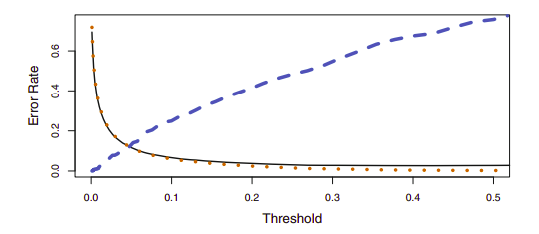
\includegraphics[width=10cm]{err-threshold.png}
\end{figure}
Using a threshold of 0.5 minimizes the overall error rate, shown as a black solid line. This is to be expected, since the Bayes classifier uses a threshold of 0.5 and is known to have the lowest overall error rate. As the threshold is reduced, the error rate among a specific classification decreases steadily (orange dotted line), but the error rate among the observations who do not belong to the class increases (blue dotted line).

Varying the classifier threshold changes its true positive and false positive rate. These are also called the sensitivity and one minus the specificity of our classifier. Below are tables of classifier names and measures.

\begin{figure}[H]
    \centering
    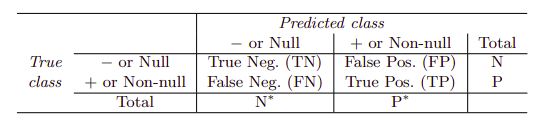
\includegraphics[width=10cm]{classifier-names.png}
\end{figure}
\begin{figure}[H]
    \centering
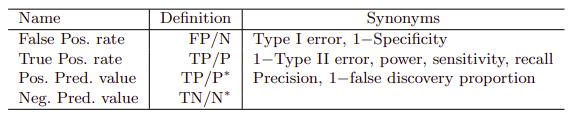
\includegraphics[width=10cm]{classifier-measures.png}
\end{figure}
The denominators for the false positive and true positive rates
are the actual population counts in each class. In contrast, the denominators for the positive predictive value and the negative predictive value are the total predicted counts for each class.
\begin{figure}[H]
    \centering
    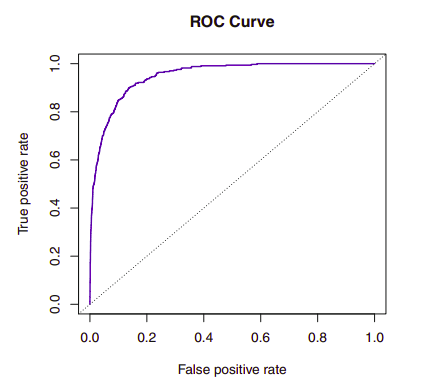
\includegraphics[width=8cm]{roc-curve.png}
\end{figure}
The \textit{ROC curve} (receiver operating characteristics) above is a popular graphic for simultaneously displaying the two types of errors for all possible thresholds. The overall performance of a classifier, summarized over all possible thresholds, is given by the \textit{area under the curve} (AUC). An ideal ROC curve will hug the top left corner, so the larger the AUC the better the classifier.

\begin{figure}[H]
    \centering
    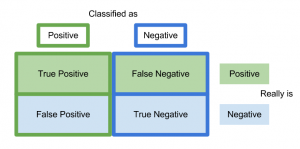
\includegraphics[width=8cm]{confusion-matrix.png}
\end{figure}

 A \textit{confusion matrix} is a way of visualizing predictions made by a classifier and is just a table showing the distribution of predictions for a specific class. The x-axis indicates the true class of each observation while the y-axis corresponds to the class predicted by the model.


\subsubsection{Quadratic Discriminant Analysis}
Similarly to LDA, the \textit{quadratic discriminant analysis} (QDA) classifier results from assuming that the observations from each class are drawn from a Gaussian distribution, and from plugging estimates for the parameters into Bayes’ theorem in order to perform prediction.  However, unlike LDA, QDA assumes that each class has its own covariance matrix, i.e. $X \sim N(\mu_k, \Sigma_k)$ where $\Sigma_k$ is a covariance matrix for the $k$th class.

Now, the Bayes classifier assigns an observation $X = x$ to the class for which $\delta_k$ is largest.
\begin{align}
\begin{split}
    \delta_k &= - \frac{1}{2}(x-\mu_k)^T \Sigma_k^{-1} (x-\mu_k) - \frac{1}{2}\log|\Sigma_k | + \log \pi_k \\
    &= - \frac{1}{2} x^T \Sigma^{-1}_k x + x^T \Sigma^{-1}_k \mu_k - \frac{1}{2} \mu_k^T \Sigma^{-1}_k  \mu_k - \frac{1}{2} \log |\Sigma_k| + \log \pi_k
\end{split}
\end{align}

The QDA classifier involves plugging estimates for $\Sigma_k, \mu_k$, and $\pi_k$ into the above equation and then assigning an observation $X = x$ to the class for which this quantity is largest. Though unlike in the LDA, the quantity $x$ appears as a quadratic function.

The reason for using QDA over LDA involves the bias-variance tradeoff. When
there are $p$ predictors, QDA must estimate $K$ covariance matrices which requires estimating $K \frac{p(p+1)}{2}$ quadratic parameters. Alternatively, LDA only estimates $Kp$ linear parameters. 

This means that LDA is a much less flexible classifier than QDA, and so has substantially lower variance, i.e. it's less prone to overfitting. This can potentially lead to improved prediction performance, but there is a trade-off: if LDA’s assumption that the $K$ classes share a common covariance matrix is badly off, then LDA can suffer from high bias. Roughly speaking, LDA tends to be a better bet than QDA if there are relatively few training observations and so reducing variance is crucial. In contrast, QDA is recommended if the training set is very large, so that the variance of the classifier is not a major concern, or if the assumption of a common covariance matrix for the $K$ classes is clearly untenable.

\subsection{A Comparison of Classification Methods}
So far we have covered 4 classification methods:  K-nearest neighbors (KNN) logistic regression, linear discriminant analysis (LDA), and quadratic discriminant analysis QDA. To describe a simple playbook: when the true decision boundaries are linear, then the LDA and logistic regression approaches will tend to perform well. When the boundaries are moderately non-linear, QDA may give better results. Finally, for much more complicated decision boundaries, a non-parametric approach such as KNN can be superior. But the level of smoothness for a non-parametric approach must be chosen carefully.

The logistic regression and LDA methods are closely connected in their linearity but differ in fitting procedures and their assumptions about the distributions in the data. To understand how, consider the two-class setting with $p = 1$ predictor, and let $p_1(x)$ and $p_2(x)=1-p1(x)$ be the probabilities that the observation $X = x$ belongs to class 1 and class 2 respectively. In the LDA framework, the log odds is given by,
\begin{equation}
    \log \Bigg( \frac{p_1(x)}{1 -p_1(x)}\Bigg) = \log \Bigg( \frac{p_1(x)}{p_2(x)}\Bigg) = c_0 + c_1 x,
\end{equation}
where $c_0$ and $c_1$ are functions of $\mu_1, \mu_2$, and $\sigma2$. In logistic regression we have,
\begin{equation}
    \log \Bigg( \frac{p_1(x)}{1 -p_1(x)}\Bigg) = \beta_0 + \beta_1 x.
\end{equation}
Both of these equations are linear functions of x so both logistic regression and LDA produce linear decision boundaries. The only difference is the fact that $\beta_0$ and $\beta_1$ are estimated using maximum likelihood, whereas $c_0$ and $c_1$ are computed using the estimated mean and variance from a normal distribution. This connection also holds for multidimensional data with $p > 1$.

Though logistic regression and LDA differ only in their fitting procedures, one may outperform the other depending on whether the LDA distribution assumptions are met, i.e. that observations are drawn from a Gaussian distribution with a common covariance matrix.

Recall that KNN is non-parametric approach: no assumptions are made about the shape of the decision boundary. Therefore, we can expect this approach to dominate LDA and logistic regression when the decision boundary is highly non-linear.  On the other hand, KNN does not tell us which predictors are important; we don’t get a table of coefficients.

Finally, QDA serves as a compromise between the non-parametric KNN method and the linear LDA and logistic regression approaches. QDA can accurately model a wider range of problems than the linear methods, and though it's not as flexible as KNN, it can perform better in the presence of a limited number of training observations because it does make some assumptions about the form of the decision boundary.

\newpage
\section{Resampling Methods}
Resampling methods involve repeatedly drawing samples from a training set and refitting a model of interest on each sample in order to obtain additional information about the fitted model. Resampling approaches can be computationally expensive, because they involve fitting the same statistical method multiple times using different subsets of the training data. However, due to recent advances in computing power, the computational requirements of resampling methods generally are not prohibitive. Two of the most commonly used resampling methods are \textit{cross-validation} and the \textit{bootstrap}.

Cross-validation can be used to estimate the test error associated with a given statistical learning method, or to select the appropriate level of flexibility. The process of evaluating a model’s performance is known as \textit{model assessment}, whereas the process of selecting the proper level of flexibility for a model is known as \textit{model selection}. The bootstrap is most commonly used to provide a measure of accuracy of a parameter estimate or of a given statistical learning method.

\subsection{Cross-Validation}
In the absence of a very large designated test set that can be used to directly estimate the test error rate some methods make a mathematical adjustment to the training error rate in order to estimate the test error rate, examined later. Alternatively, we now consider a class of methods that estimate the test error rate by holding out a subset of the training observations from the fitting process, and then applying the statistical learning method to those held out observations.

\subsubsection{The Validation Set Approach}
The \textit{validation set approach}  is a very simple strategy that involves randomly dividing the available set of observations into two parts, a \textit{training set} and a \textit{validation set} or hold-out set. The model is fit on the training set, and the fitted model is used to predict the responses for the observations in the validation set which provides an estimate of the test error rate.

The validation set approach has two potential drawbacks which will be addressed in cross-validation:
\begin{enumerate}
    \item The validation estimate of the test error rate can be highly variable, depending on precisely which observations are included in the training set and which observations are included in the validation set.
    \item In the validation approach, only a subset of the observations that are included in the training set are used to fit the model. This suggests that the validation set error rate may tend to overestimate the test error rate.
\end{enumerate}

\subsubsection{Leave-One-Out Cross-Validation}
\textit{Leave-one-out cross-validation} (LOOCV) also involves splitting the set of observations into two parts but instead of creating two subsets of comparable size, a single observation $(x_1, y_1)$ is used for the validation set, and the remaining observations $\{(x_2, y_2),...,(x_n, y_n)\}$ make up the training set. 

Although $MSE_1 = (y_1 - \hat y_1)^2$ provides an approximately unbiased estimate for the test error, it is a poor estimate because it is highly variable since it is based upon a single observation. We can repeat the procedure by selecting $(x_2, y_2)$  for the validation data, training the statistical learning procedure on the other $n - 1$ observations, repeating this approach $n$ times. The LOOCV estimate for the test MSE is the average of these $n$ test error
estimates:
\begin{equation}
     CV_{(n)} = \frac{1}{n} \sum_{i=1}^n MSE_i.
\end{equation}
Using all but one of the observations for training results in less bias and tends not to overestimate the test error rate as much as the validation set approach does. in contrast to the validation approach, performing LOOCV multiple times will always yield the same results: there is no randomness in the training/validation set splits.

LOOCV can be expensive and time consuming if $n$ is large or the model is slow to fit since the model has to be fit $n$ times. With least squares linear or polynomial regression, an amazing shortcut makes the cost of LOOCV the same as that of a single model fit.
\begin{equation}
     CV_{(n)} = \frac{1}{n} \sum_{i=1}^n \Bigg ( \frac{y_i-\hat y_i}{1-h_i} \Bigg )^2.
\end{equation}
where $\hat y_i$ is the $i$th fitted value from the original least squares fit, and $h_i$ is the leverage defined previously \eqref{eq:leverage}. This is like the ordinary MSE, except the ith residual is divided by $1 - h_i$ The leverage lies between $1/n$ and $1$, and reflects the amount that an observation influences its own fit. Hence the residuals for high-leverage points are inflated in this formula by exactly the right amount for this equality to hold. LOOCV is a very general method, and can be used with any kind of predictive modeling.

\subsubsection{k-Fold Cross-Validation}
\textit{k-fold CV} involves randomly dividing the set of observations into k groups, or folds, of approximately equal size.  The first fold is treated as a validation set, and the method is fit on the remaining $k - 1$ folds, then the mean squared error is computed on the held-out fold. This is repeated $k$ times on different groups of observations.
\begin{equation}
    CV_{(k)} = \frac{1}{k} \sum_{i=1}^k MSE_i.
\end{equation}
LOOCV is a special case of k-fold CV in which $k$ equals $n$. In practice, one typically performs k-fold CV using k = 5 or k = 10 depending on computational costs and the bias-variance trade-off. 
The actual estimate of the test MSE is may not be of interest, and we're instead interested in only in the location of
the minimum point in the estimated test MSE curve corresponding to the correct flexibility level.

\subsubsection{Bias-Variance Trade-Off for k-Fold Cross-Validation}

A more important advantage of k-fold CV is that it often gives more accurate estimates of the test error rate than does LOOCV. This has to do with a bias-variance trade-off. Since LOOCV trains on $n-1$ observations, it seems preferable to  k-fold CV from the perspective of bias reduction. However, we must also consider the procedure’s variance. It turns out that LOOCV has higher variance than does k-fold CV with $k<n$.

When we perform LOOCV, we are in effect averaging the
outputs of $n$ fitted models, each of which is trained on an almost identical set of observations; therefore, these outputs are highly (positively) correlated with each other. In contrast, with k-fold CV we are averaging the outputs of k fitted models that are somewhat less correlated with each other, since the overlap between the training sets in each model is smaller. Since the mean of many highly correlated quantities has higher variance than does the mean of many quantities that are not as highly correlated, the test error estimate resulting from LOOCV tends to have higher variance.

\subsubsection{Cross-Validation on Classification Problems}
Cross-validation can also be a very useful approach in the classification setting when $Y$ is qualitative. Rather than using MSE to quantify test error, we instead use the number of misclassified observations. The LOOCV error rate becomes,
\begin{equation}
    CV_{(n)} = \frac{1}{n}\sum_{i=1}^n Err_i,
\end{equation}
where $Err_i = I(y_i \neq \hat y_i)$. The k-fold CV error rate and validation set error rates are defined analogously.

\subsection{ The Bootstrap}
The \textit{bootstrap} can be used to quantify the uncertainty associated with a given estimator or statistical learning method, some for which a measure of variability is otherwise difficult to obtain and is not automatically output by
statistical software.

the bootstrap approach allows us to use a computer to emulate the process of obtaining new sample sets. s. Rather than repeatedly obtaining independent data sets from the population, we instead obtain distinct data sets by repeatedly sampling observations from the original data set.

Given a simple data set $Z$ that contains $n$ observations, We randomly select $n$ observations from the data set in order to produce a bootstrap data set, $Z^{*1}$.  The sampling is performed with \textit{replacement}, which means that the same observation can occur more than once. This procedure is repeated $B$ times for some large value of $B$, in order to produce
$B$ different bootstrap data sets, $Z^{*1}, Z^{*2},\dots,Z^{*B}$ and $B$ corresponding $\alpha$ estimates, $\hat \alpha^{*1},\dots, \hat \alpha^{*B}$. We can compute the standard error of these bootstrap estimates using the formula,
\begin{equation}
    \text{SE}_B(\hat \alpha) = \sqrt{\frac{1}{B-1} \sum_{r=1}^{B} \Bigg ( \hat \alpha ^{*r} - \frac{1}{B} \sum_{r'=1}^{B} \hat \alpha^{*r'} \Bigg )^2 } .  
\end{equation}


\newpage
\section{Linear Model Selection and Regularization}
Alternative fitting procedures to least squares can yield better prediction accuracy and model interpretability.

Prediction Accuracy -- If $n$, the number of observations, is much larger than $p$, the number of variables, i.e. $n >>p$, then the least squares estimates tend to have low variance and will perform well on test observations. If $n$ is not much larger than $p$, then there can be a lot of variability in the least squares fit, resulting in overfitting and poor predictions on unseen future observations. If $p>n$, then there is no longer a unique least squares coefficient estimate: the variance is infinite so the method cannot be used at all.

Model Interpretability -- Often some or many of the variables used in a multiple regression model are not associated with the response and their inclusion leads to unnecessary complexity in the resulting model. By setting the corresponding coefficient estimates to zero, we can obtain a model that is more easily interpreted. However, least squares is extremely unlikely to yield any coefficient estimates that are exactly zero. There exist alternative approaches for automatically performing \textit{feature selection} or \textit{variable selection}.

\begin{enumerate}
    \item Subset Selection -- This approach involves identifying a subset of the p predictors that we believe to be related to the response. We then fit a model using least squares on the reduced set of variables.
    
    \item Shrinkage --  This approach involves fitting a model involving all p predictors. However, the estimated coefficients are shrunken towards zero relative to the least squares estimates which has the effect of reducing variance. Some coefficients may be estimated to be exactly zero, resulting in variable selection.
    
    \item Dimension Reduction -- This approach involves projecting the $p$ predictors into a M-dimensional subspace, where $M<p$. This is achieved by computing $M$ different linear combinations, or projections, of the variables. Then these $M$ projections are used as predictors to fit a linear regression model by least squares.
    
\end{enumerate}

\subsection{Subset Selection}
\subsubsection{Best Subset Selection}
To perform \textit{best subset selection}, we fit a separate least squares regression for each possible combination of the $p$ predictors. That is, we fit all $p$ models that contain exactly one predictor, then all $\binom{p}{2}= p(p-1)/2$ models that contain exactly two predictors, and so forth up to $\binom{p}{2}$ . We then try to identify the one that is best model out of the $2^p$ possibilities. Here best is defined as having the smallest RSS, or equivalently largest $R^2$.

The algorithm is as follows:
\begin{enumerate}
    \item Let $M_0$ denote the null model, which contains no predictors. This model simply predicts the sample mean for each observation.
    \item For $k = 1, 2,...p$:
    \begin{enumerate}
        \item Fit all $\binom{p}{k}$ models that contain exactly $k$ predictors.
        \item Pick the best  among these $\binom{p}{k}$ models, and call it $M_k$. Here best is defined as having the smallest RSS, or equivalently largest $R^2$.
    \end{enumerate}
    \item Select a single best model from among $M_0,\dots,M_p$ using cross-validated prediction error, $C_p$ (AIC), BIC, or adjusted $R^2$.
\end{enumerate}

As the number of features included in the models increases, the RSS of these $p + 1$ models decreases monotonically, and the $R^2$ increases monotonically which indicates a model with a low training error, whereas we wish to choose a model that has a low test error. So if we use these statistics to select the best model, then we will always end up with a model involving all of the variables. This is why in in Step 3, we use cross-validated prediction error in order to select among the models.

The same ideas used with least squares applies to other types of models, such as logistic regression, where instead of ordering models by RSS in Step 2, we use the \textit{deviance}, a measure that plays the role of RSS for a broader class of models. The deviance is negative two times the maximized log-likelihood; the smaller the deviance, the better the fit. 

Best subset selection becomes computationally infeasible for values of $p$ greater than around 40.

\subsubsection{Stepwise Selection}
An enormous search space can lead to overfitting and high variance of the coefficient estimates which makes \textit{stepwise} methods, which explore a far more restricted set of models, an attractive alternative to best subset selection.

\subsubsection*{Forward Stepwise Selection}
Forward stepwise selection considers a much smaller set of models. begins with a model containing no predictors, and then adds predictors to the model, one-at-a-time, until all of the predictors are in the model. In particular, at each step the variable that gives the greatest additional improvement to the fit is added to the model.
\begin{enumerate}
    \item Let $M_0$ denote the null model, which contains no predictors.
    \item For $k = 1, 2,...p$:
    \begin{enumerate}
        \item Consider all $p - k$ models that augment the predictors in $M_k$ with one additional predictor.
        \item  Choose the best among these $p - k$ models, and call it $M_{k+1}$. Here best is defined as having smallest RSS or highest $R^2$.
    \end{enumerate}
    \item Select a single best model from among $M_0,\dots,M_p$ using cross-validated prediction error, $C_p$ (AIC), BIC, or adjusted $R^2$.
\end{enumerate}

This amounts to a total of $1 +\sum_{k=0}^{p-1} (p-k) = 1 + p(p-1)/2$ models, though it is not guaranteed to find the best possible model out of all $2^p$ models containing subsets of the $p$ predictors.  In Step 3, we must identify the best model among a set of models with different numbers of variables, presenting some challenges.

Forward stepwise selection can be applied even in the high-dimensional setting where $n<p$; however, in this case, it is possible to construct submodels $M_0,\dots,M_{n-1}$ only, since each submodel is fit using least squares, which will not yield a unique solution if $p \geq n$.

\subsubsection*{Backward Stepwise Selection}
Unlike forward stepwise selection, \textit{backward stepwise selection} begins with the full least squares model containing all $p$ predictors, and then iteratively removes the least useful predictor, one-at-a-time.
\begin{enumerate}
    \item Let $M_0$ denote the null model, which contains no predictors.
    \item For $k = p, p-1,...1$:
    \begin{enumerate}
        \item Consider all $k$ models that contain all but one of the predictors in $M_k$, for a total of $k-1$ predictors.
        \item  Choose the best among these $k$ models, and call it $M_{k+1}$. Here best is defined as having smallest RSS or highest $R^2$.
    \end{enumerate}
    \item Select a single best model from among $M_0,\dots,M_p$ using cross-validated prediction error, $C_p$ (AIC), BIC, or adjusted $R^2$.
\end{enumerate}

This produces the same number of models as forward selection, i.e. $1 +\sum_{k=0}^{p-1} (p-k)$, and is also not guaranteed to yield the best model containing a subset of the $p$ predictors.

\subsubsection*{Hybrid Approaches}
Hybrid versions of forward and backward stepwise selection are available, in which variables are added to the model sequentially, as in forward selection, and after adding each new variable, the method may also remove any variables that no longer provide an improvement in the model fit, as in backward selection.

\subsubsection{Choosing the Optimal Model}
If we wish to choose a model with a low test error, the training error can be a poor estimate of the test error. Therefore, RSS and $R^2$ are not suitable for selecting the best mode among a collection of models with different numbers of predictors. There are two common approaches to estimate this test error:
\begin{enumerate}
    \item We can indirectly estimate test error by making an adjustment to the training error to account for the bias due to overfitting.
    \item  We can directly estimate the test error, using either a validation set approach or a cross-validation approach.
\end{enumerate}

\subsubsection*{\texorpdfstring{$C_p$}{Cp}, AIC, BIC, and Adjusted \texorpdfstring{$R^2$}{ R2}}
Using least squares, we  estimate the regression coefficients such that the training RSS (but not the test RSS) is as small as possible. So the training error will decrease as more variables are included in the model, but the test error may not. We now consider four alternative approaches: $C_p$, \textit{Akaike information criterion} (AIC), \textit{Bayesian information criterion} (BIC), and \textit{adjusted $R^2$}.

For a fitted least squares model containing d predictors, the $C_p$ estimate of test MSE is computed using the equation,
\begin{equation}
    C_p = \frac{1}{n}(RSS + 2d\hat\sigma^2)
\end{equation}
where $\hat\sigma2$ is an unbiased estimate of the variance of the error $\epsilon$ associated with each response measurement in the standard linear model. Essentially, the $C_p$ statistic adds a penalty of $2d\hat\sigma^2$ to the training RSS in order to adjust for the fact that the training error tends to underestimate the test error, where the penalty increases as the number of predictors in the model increases. When determining which of a set of models is best, we choose the model with the lowest $C_p$ value.

The AIC criterion is defined for a large class of models fit by maximum
likelihood In the case of the model with Gaussian errors, maximum likelihood and least squares are the same thing. In this case AIC is given by

\begin{equation}
    AIC = \frac{1}{n\hat\sigma^2} (RSS + 2d\hat\sigma^2)
\end{equation}

BIC is derived from a Bayesian point of view, but ends up looking similar
to $C_p$ (and AIC) as well. For the least squares model with $d$ predictors, the
BIC is, up to irrelevant constants, given by
\begin{equation}
    BIC = \frac{1}{n \hat\sigma^2} (RSS  + \log(n)d\hat\sigma^2)
\end{equation}
Like $C_p$, we select the model that has the lowest BIC value.  Since $\log n > 2$ for any $n > 7$, the BIC statistic generally places a heavier penalty on models with many variables.

The adjusted $R^2$ statistic is another popular approach for selecting among a set of models that contain different numbers of variables. Recall the usual $R^2$ is defined as $1 - RSS/TSS$, which always decreases as more variables are added to the mode. For a least squares model with $d$ variables, the adjusted $R^2$ statistic is calculated as,
\begin{equation}
\text{Adjusted }R^2 = 1 - \frac{RSS/(n-d-1)}{TSS/(n-1)}
\end{equation}
Here, a large value of adjusted $R^2$ indicates a model with a small test error. The intuition behind the adjusted R2 is that once all of the correct variables have been included in the model, adding additional noise variables will increase d and increase the denominater while only leading to only a very small decrease in RSS.

\subsubsection*{Validation and Cross-Validation}
AIC, BIC, and $C_p$  can also be defined for more general types of models. As an alternative to the approaches just discussed, We can compute the validation set error or the cross-validation error for each model under consideration, and then select the model for which the resulting estimated test error is smallest. This has the advantage of providing a direct estimate of the test error, and makes fewer assumptions about the true underlying model. It can also be used in a wider range of model selection tasks where it is hard to pinpoint the model
degrees of freedom i.e. predictors, or to estimate the error variance $\sigma^2$. 

In the \textit{one-standard-error rule}, we first calculate the standard error of the estimated test MSE for each model size, and then select the smallest model for which the estimated test error is within one standard error of the lowest point on the curve. The rationale here is that if a set of models appear to be more or less equally good, then we might as well choose the simplest model—that is, the model with the smallest number of predictors.

\subsection{Shrinkage Methods}
As an alternative, we can fit a model containing all $p$ predictors using a technique that constrains or regularizes the coefficient estimates, or equivalently, that shrinks the coefficient estimates towards zero, which can significantly reduce their variance. The two best-known techniques for shrinking the regression coefficients towards zero are ridge regression and the lasso

\subsubsection{Ridge Regression}
Recall the least squares fitting procedure estimates coefficients $\beta_j$ that minimize the RSS \eqref{eq:RSS}. Similarly, \textit{Ride Regression} estimates the coefficients $B^R$ that minimize,
\begin{equation}
    RSS + \lambda + \lambda \sum_{j=1}^{p} \beta_j^2  
    = \sum_{i=1}^{n} \Bigg( y_i - \beta_0 - \sum_{j=1}^{p} \beta_j x_{ij} \Bigg )^2  
    + \lambda \sum_{j=1}^{p} \beta_j^2,
\end{equation}
where $\lambda \geq 0$ is a \textit{tuning parameter}, to be determined separately. the second term $\lambda \sum \beta_j^2$, called a \textit{shrinkage penalty}, is small when $\beta_1,\dots,\beta_p$ are close to zero, and so it has the effect of shrinking the estimates of $\beta_j$ towards zero. The tuning parameter $\lambda$ serves to control the relative impact of these two terms on the regression coefficient estimates excluding the intercept coefficient $\beta_0$. Ridge regression will produce a different set of coefficient estimates, $\beta^R_\lambda$, for each value of $\lambda$, so selecting a good value tuning parameter via cross validation is critical.

The value $X_j\beta^R_{j,\lambda}$ will not only depend on the value of $\lambda$, but also on the scaling of the $j$th predictor. In fact, the value of $X_j\beta^R_{j,\lambda}$ may even depend on the scaling of the other predictors. Therefore, it is best to apply ridge regression after standardizing the predictors by applying the estimated standard deviation of the $j$th predictor with the formula,
\begin{equation}
    \Tilde{x_{ij}} = \frac{x_{ij}}{\sqrt{\frac{1}{n} \sum{i=1}^{n} (x_{ij} - \bar x_j)^2}}.
\end{equation}
Ridge regression’s advantage over least squares is rooted in the bias-variance trade-of. As $\lambda$ increases, the flexibility of the ridge regression fit decreases, leading to decreased variance but increased bias. This leads to a decrease in the  mean squared error (MSE), which is a function of the variance plus the squared bias.

When the number of variables $p$ is almost as large as the number of observations $n$, the least squares estimates will be extremely variable. And if $p>n$, then the least squares estimates do not even have a unique solution, whereas ridge regression can still perform well by trading off a small increase in bias for a large decrease in variance.  Hence, ridge regression works best in situations where the least squares estimates have high variance.

Though the penalty can shrink some of the coefficients towards zero, ridge regression will include all $p$ predictors in the final model. This can create a challenge in model interpretation

\subsubsection{The Lasso}
The \textit{lasso} is a relatively recent alternative to ridge regression that overcomes the disadvantage of uninterpretable models with a large number of predictors. The lasso coefficients, $ \Tilde{\beta^L_\lambda}$, minimize the quantity
\begin{equation}
    RSS + \lambda \sum_{j=1}^{p} |\beta_j| 
    = \sum_{i=1}^{n} \Bigg( y_i - \beta_0 - \sum_{j=1}^{p} \beta_j x_{ij} \Bigg )^2 +  \lambda \sum_{j=1}^{p} |\beta_j| .
\end{equation}
The difference between ridge regression and lasso is the penalty $\beta_j^2$ has been replaced with $|\beta_j|$. The lasso uses an $\ell_1$ (pronounced ``ell 1") penalty instead of an $\ell_2$ penalty. The $\ell_1$ norm of a coefficient vector $\beta$ is given by $||\beta||_1 = \sum |\beta_j|$. This has the effect of forcing some of the coefficient estimates to be exactly equal to zero when the tuning parameter $\lambda$ is sufficiently large. Thus, the lasso performs variable selection, resulting in more interpretable and \textit{sparse} models, involving only a subset of the variables.

\subsubsection*{The Variable Selection Property of the Lasso}
When we perform the lasso we are trying to find the set of coefficient estimates that lead to the smallest RSS, subject to the constraint that there is a budget $s$ for how large 
$\sum_{j=1}^p |\beta_j |$ can be. Ridge regression more or less shrinks every dimension of the data by the same proportion, whereas the lasso more or less shrinks all coefficients toward zero by a similar amount, and sufficiently small coefficients are shrunken all the way to zero, known as \textit{soft thresholding}.


\subsubsection*{Comparing the Lasso and Ridge Regression}
Neither ridge regression nor the lasso will universally dominate the other. In general, one might expect the lasso to perform better in a setting where a relatively small number of predictors have substantial coefficients, and the remaining predictors have coefficients that are very small or that equal zero. Ridge regression will perform better when the response is a function of many predictors, all with coefficients of roughly equal size. However, the number of predictors that is related to the response is never known a priori for real data sets. A technique such as cross-validation can be used in order to determine which approach is better on a particular data set.

\subsubsection*{Bayesian Interpretation for Ridge Regression and the Lasso}
A Bayesian viewpoint for regression assumes that the coefficient vector $\beta$ has some prior distribution, say $p(\beta)$, where $\beta = (\beta_0, \dots, \beta_p )^T$. The likelihood of the data is $f(Y |X, \beta)$ where $X= (X_1, \dots, X_p)^T$.  Multiplying the prior distribution by the likelihood gives us the \textit{posterior distribution},
\begin{equation}
    p(\beta|X, Y ) \propto f(Y |X, \beta) p(\beta|X) = f(Y |X, \beta)p(\beta),
\end{equation}
which follows from Bayes’ theorem. We assume the usual linear model, and suppose that the errors are independent and drawn from a normal distribution. We also assume $p(\beta) = \prod^{p}+{j=1} g(\beta_j)$, for some density function $g$. Then,  ridge regression and the lasso follow from two special cases of $g$:
\begin{enumerate}
    \item If $g$ is a Gaussian distribution with mean zero and standard deviation a function of $\lambda$, then it follows that the posterior mode for $\beta$, i.e. the most likely value for $\beta$, given the data, is given by the ridge regression solution.
    
    \item If $g$ is a double-exponential (Laplace) distribution with mean zero and scale parameter a function of $\lambda$, then it follows that the posterior mode for $\beta$ is the lasso solution.
\end{enumerate}

\subsubsection{Selecting the Tuning Parameter}
Implementing ridge regression and the lasso requires a method for selecting a value for the tuning parameter $\lambda$.  Cross-validation provides a simple way to tackle this problem. We choose a grid of $\lambda$ values, and compute the cross-validation error for each value of $\lambda$. We then select the tuning parameter value for which the cross-validation error is smallest. Finally, the model is re-fit using all of the available observations and the selected value of the tuning parameter.


\subsection{Dimension Reduction Methods}
\textit{Dimension reduction methods} transform the predictors and then fit a least squares model using the transformed variables. Let $Z_1, Z_2,\dots, Z_M$ represent $M<p$ linear combinations of our original $p$ predictors. That is,
\begin{equation}
    Z_m = \sum_{j=0}^p \phi_{jm}X_j
\end{equation}
for some constants $\phi_{1m}, \phi_{2m},\dots,\phi_{pm}, m = 1,...,M$. We can then fit the linear regression model,
\begin{equation}
    y_i = \theta_0 + \sum_{m=1}^M \theta_m z_{im} + \epsilon_i, \ \ i = 1,\dots, n
\end{equation}
using least squares, which can possibly outperform the standard linear model with wisely chosen coefficients. The term dimension reduction comes from the fact that this approach reduces the problem of estimating the $p+1$ to $M+1$ coefficients, where $M < p$. The model can be thought of as a special case of the linear model, with coeffecients $\theta_m$ being related by $\beta_j = \sum_{m=1}^M \theta_m \phi_{jm}$. Methods for obtaining the tranformed predictors are examined next.

\subsubsection{Principal Component Regression}
\textit{Principal components analysis} (PCA) is a popular approach for deriving a low-dimensional set of features from a large set of variables and is examined in more detail later. PCA is a technique for reducing the dimension of a $n \times n$ data matrix $X$.

The first principal component, $Z_1$, moves along the  data in the direction which the observations vary the most, where directions corresponds to linear combinations. Alternatively, we can think of the first principal component as a vector that defines the line that is as close as possible to the data. The first principal component score measures this distance by selecting linear combinations of $X_i, X_j$ predictors with $\sigma_{11}^2 + \sigma_{21}^2 = 1$ that yield the highest variance. With two-dimensional data and two predictors $X_1, X_2$, this looks like,
\begin{equation}
    Z_1 = Var(\sigma_{11} \times (X_1 - \bar X )  + \sigma_{21} \times (X_2  - \bar X)).
\end{equation}
The second principal component $Z^2$ is a linear combination of the variables that are uncorrelated with $Z^1$, and has largest variance subject to this constraint, i.e. the direction must be perpendicular, or perpendicular orthogonal, to the first principal component direction.
\begin{equation}
    Z_2 = Var(\sigma_{21} \times (X_1 - \bar X )  + \sigma_{11} \times (X_2  - \bar X)) 
\end{equation}
With more predictors, additional components could be constructed.  They would successively maximize variance, subject to the constraint of being uncorrelated with the preceding components.

\subsubsection*{The Principal Components Regression Approach}

The \textit{principal components regression} (PCR) approach involves constructing the first $M$ principal components, $Z_1,\dots,Z_M$, and then using these components as the predictors in a linear regression model that is fit using least squares.  Often a small number of principal components suffice to explain most of the variability in the data, as well as the relationship with the response, i.e. the directions in which $X_1,...,X_p$ show the most variation are the directions that are associated with $Y$. If this assumption holds, our PCR model will lead to better results since using less coefficients will mitigate overfitting. PCR will tend to do well in cases when the first few principal components are sufficient to capture most of the variation in the predictors as well as the relationship with the response.

Yet PCR is not considered a feature selection method, since the $M$ principal components used in the regression is a linear combination of all $p$ of the original features. In this sense, PCR is more closely related to ridge regression than to the lasso, where ridge regression can be thought of as a continuous version of PCR. It's recommended to standardize each predictor prior to generating the principal components with PCR because high-variance variables will tend to play a larger role in the principal components obtained

The directions or linear combinations are identified in an unsupervised way, since the response $Y$ is not used to help determine or supervise the indentification of the principal component directions. Consequently, PCR suffers from the drawback that there is no guarantee that the
directions that best explain the predictors will also be the best directions to use for predicting the response.

\subsubsection{Partial Least Squares}

\textit{Partial least squares} (PLS) is a supervised alternative to PCR. That is, PLS is also a dimension reduction method which identifies a set of features that are linear combinations of the original features and then fits a linear model via least squares. But unlike PCR, PLS uses a supervised method to identifiy features that not only approximate the old features well, but also that are related to the response by attempting to find directions that help explain both the response and the predictors.

After standardizing the p predictors,  PLS computes the first direction $Z_1$ by setting each $\phi_{j1}$ in the dimension reduction features equal to the coefficient from the simple linear regression of $Y$ onto $X_j$. One can show that this coefficient is proportional to the correlation between $Y$ and $X_j$. Hence, in computing $Z_1 = \sum_{j=1}^{p} \phi_{j1}X_j$, PLS places the highest weight on the variables that are most strongly related to the response.

To identify the second PLS direction we first adjust each of the variables for $Z_1$, by regressing each variable on $Z_1$ and taking residuals. These residuals can be interpreted as the remaining information that has not been explained by the first PLS direction. We then compute $Z_2$ using this orthogonalized data in exactly the same fashion as $Z_1$ was computed based on the original data. This iterative approach can be repeated $M$ times to identify multiple PLS components $Z_1,\dots,Z_M$. Finally, at the end of this procedure, we use least squares to fit a linear model to predict $Y$ using $Z_1,\dots,Z_M$ in exactly the same fashion as for PCR. As with PCR, the number $M$ of partial least squares directions used in
PLS is a tuning parameter that is typically chosen by cross-validation.

In practice PLS often performs no better than ridge regression or PCR. While the supervised dimension reduction of PLS can reduce bias, it also has the potential to increase variance.

\subsection{Considerations in High Dimensions}
\subsubsection{High-Dimensional Data}

A \textit{low-dimensional} setting is one in which $n$, the number of observations, is much greater than $p$, the number of features, i.e. $n>>p$.

Data sets containing more features than observations are often referred to as \textit{high-dimensional}. Classical approaches such as least squares linear regression are not appropriate in this setting. Challenges like the bias-variance trade-off and the danger of overfitting are still relevant and can become particularly important in this setting.


\subsubsection{What Goes Wrong in High Dimensions?}

When the number of features $p$ is as large as, or larger than, the number of observations n, least squares should not be performed. Regardless of whether or not there truly is a relationship between the features and the response, least squares will yield a set of coefficient estimates that result in a perfect fit to the data, such that the residuals are zero.  When $p>n$ or $p \approx n$, a simple least squares regression line is too flexible and hence overfits the data.

Care must be taken when analyzing data sets with a large number of variables, accurate evaluations of models performance must be done on an independent test set, otherwise the training set MSE can create false confidence.

Additionally, techniques visited earlier, like $C_p$, AIC, and BIC, which were useful for adjusting the training set RSS or $R^2$ in order to account for the number of variables used to fit a least squares model are also not appropriate in the high-dimensional setting. This is because estimating $\hat\sigma^2$ can be problematic and one can easily obtain a model with an adjusted $R^2$ value of 1.

\subsubsection{Regression in High Dimensions}

We can avoid overfitting by using a less flexible fitting approach
than least squares. Forward stepwise selection, ridge
regression, the lasso, and principal components regression, are particularly useful for performing regression in the high-dimensional setting

We find that (1) regularization or shrinkage plays a key role in high-dimensional problems, (2) appropriate tuning parameter selection is crucial for good predictive performance, and (3) the test error tends to increase as the dimensionality of the problem
(i.e. the number of features or predictors) increases, unless the additional features are truly associated with the response) this is also known as the curse of dimensionality. noise features increase the dimensionality of the problem, exacerbating the risk of overfitting.  Even if excess features are relevant, the variance incurred in fitting their coefficients may outweigh the reduction in bias that they bring.


\subsubsection{Interpreting Results in High Dimensions}
In the high-dimensional setting, the multicollinearity problem is extreme: any variable in the model can be written as a linear combination of all of the other variables in the model. This
means that we can never know exactly which variables truly are predictive of the outcome, and we can never identify the best coefficients for use in the regression and can only hope to assign appropriate regression coefficients to correlated variables.

As mentioned before, one should never use sum of squared errors, p-values, $R^2$ statistics  or other traditional measures of model fit on the training data as evidence of a good model fit in the high-dimensional setting. It is important to instead report results on an independent test set, or cross-validation errors. For instance, the MSE or $R^2$ on an independent test set is a valid measure of model fit, but the MSE on the training set is not.



\newpage
\section{Moving Beyond Linearity}
Although However, standard linear regression can have  have advantages over other approaches in terms of interpretation and inference, it has significant limitations in terms of predictive power because the linearity assumption is almost always an approximation, and sometimes a poor one. 

\begin{itemize}
    \item \textit{Polynomial regression} extends the linear model by adding extra predictors, obtained by raising each of the original predictors to a power. This approach provides a simple way to provide a nonlinear fit to data.
    \item \textit{Step functions} cut the range of a variable into $K$ distinct regions in order to produce a qualitative variable. This has the effect of fitting a piecewise constant function.
    \item \textit{Regression splines} are more flexible than polynomials and step functions, and in fact are an extension of the two. They involve dividing the range of X into K distinct regions. Within each region, a polynomial function is fit to the data. However, these polynomials are constrained so that they join smoothly at the region boundaries, or knots. Provided that the interval is divided into enough regions, this can produce an extremely flexible fit.
    \item Smoothing splines are similar to regression splines, but arise in a slightly different situation. Smoothing splines result from minimizing a residual sum of squares criterion subject to a smoothness penalty.
    \item Local regression is similar to splines, but differs in an important way. The regions are allowed to overlap, and indeed they do so in a very smooth way.
    \item Generalized additive models allow us to extend the methods above to deal with multiple predictors.
\end{itemize}
\subsection{Polynomial Regression}
Historically, the way to extend linear regression was to replace the standard linear model,
\[
    y_i = \beta_0 + \beta_1 x_i + \epsilon_i
\]
with with a polynomial function,
\begin{equation}
    y_i = \beta_0 + \beta_1 x_i + \beta_2 x_i^2 + \dots + \beta_d x_i^d + \epsilon_i
\end{equation}
in an approach known as \textit{polynomial regression}. Using a large enough degree $d$, a polynomial regression allows us to produce an extremely non-linear curve but in General, it is unusual
to use $d$ greater than 3 or 4 because for large values of d, the polynomial curve can become overly flexible and can take on some very strange shapes. This is especially true near the boundary of the $X$ variable.

\subsection{Step Functions}
Using polynomial functions of the features as predictors in a linear model imposes a global structure on the non-linear function of X. We can instead use \textit{step functions} in order to avoid imposing such a global structure. We break the range of $X$ into bins, and fit a different constant in each bin. This amounts to converting a continuous variable into an \textit{ordered categorical variable}.

We create cutpoints $c_1, c_2,\dots,c_K$ in the range of $X$, and then construct $K + 1$ new variables, sometimes called \textit{dummy variables},
\begin{align}
\begin{split}
    C_0(X) &= I(X<c_1), \\
    C_1(X) &= I(c_1 \leq X < c_2),\\
    C_2(X) &= I(c_2 \leq X<c_3),\\
    &\vdots \\
    C_{K-1}(X) &= I(c_{K-1} \leq X < c_K),\\
    C_K(X) &= I(c_K \leq X),
\end{split}
\end{align}
where $I()$ is an \textit{indicator function} that returns a 1 if the condition is true, and 0 otherwise. Notice that for any value of $X$, $C_0(X) + C_1(X) + \dots + C_K(X) = 1$, since $X$ must
be in exactly one of the $K + 1$ intervals. We then use least squares to fit a linear model using $C_1(X), C_2(X),\dots,C_K(X)$ as predictors:
\begin{equation}
    y_i = \beta_0 + \beta_1C_1(x_i) + \beta_2C_2(x_i) + \dots + \beta_KC_K(x_i) + i.
\end{equation}
Note that when $X<c_1$, all of the predictors in the above equation are zero, so $\beta_0$ can be interpreted as the mean value of $Y$ for $X<c_1$. Then the model predicts a response of $\beta_0+\beta_j$ for $c_j \leq X<c_j+1$. So $\beta_j$ represents the average increase in the response for $X$ in $c_j \leq X<c_j+1$ relative to $X<c_1$.

Unfortunately, unless there are natural breakpoints in the predictors, piecewise-constant functions can miss the action. Nevertheless, step function approaches are very popular in biostatistics and epidemiology, among other disciplines. For example, 5-year age groups are often used to define the bins.

\subsection{Basis Functions}
Polynomial and piecewise-constant regression models are in fact special cases of a \textit{basis function} approach. The idea is to have at hand a family of functions or transformations that can be applied to a variable $X$: $b_1(X), b_2(X),\dots, b_K(X)$. Instead of fitting a linear model in $X$, we fit the model
\begin{equation}
    y_i = \beta_0 + \beta_1b_1(x_i) + \beta_2b_2(x_i) + \dots + \beta_Kb_K(x_i) + \epsilon_i.
\end{equation}
Note that the basis functions $b_1(), b_2(),\dots,b_K()$ are fixed and known ahead of time. We can think of the model as a standard linear model with predictors $b_1(x_i), b_2(x_i),\dots, b_K(x_i)$. Hence, we can use least squares to estimate the unknown regression coefficients in the model. Importantly, this means that all of the inference tools for linear models, such as standard errors for the coefficient estimates and F-statistics for the model’s overall significance, are also available in this setting.

For polynomial regression, the basis functions are $b_j(x_i) = x_i^j$, and for piecewise constant functions they are $b_j (x_i) = I(c_j \leq x_i < c_{j+1})$. Many alternatives for our basis functions are possible like wavelets or Fourier series or the very common choice of regression splines.

\subsection{Regression Splines}
\textit{Regression splines} are a flexible class of basis functions that extends upon the polynomial regression and piecewise constant regression approaches.

\subsubsection{Piecewise Polynomials}

\subsubsection{Constraints and Splines}
\subsubsection{The Spline Basis Representation}
\subsubsection{Choosing the Number and Locations of the Knots}
\subsubsection{Comparison to Polynomial Regression}

\subsection{Smoothing Splines}
\subsubsection{An Overview of Smoothing Splines}
\subsubsection{Choosing the Smoothing Parameter \texorpdfstring{$\lambda$}{lambda}}

\subsection{Local Regression}

\subsection{Generalized Additive Models}
\subsubsection{GAMs for Regression Problems}
\subsubsection{GAMs for Classification Problems}



\newpage
\section{Tree-based Methods}

\newpage
\section{Support Vector Machines}

\newpage
\section{Unsupervised Learning}

\end{enumerate}


\comment{
- left off: pg 47, video:  Lect3 4b 110613
- 
}


\newpage
\begin{thebibliography}{}
\bibitem[]{}
Gareth James, Daniela Witten, Trevor Hastie, Robert Tibshirani. An Introduction to Statistical Learning : with Applications in R. New York :Springer, 2013.


http://faculty.marshall.usc.edu/gareth-james/ISL/ISLR\%20Seventh\%20Printing.pdf

% https://www.dataschool.io/15-hours-of-expert-machine-learning-videos/


\bibitem[]{}
https://arxiv.org/pdf/1010.3162.pdf

\bibitem[]{}
http://bactra.org/notebooks/learning-theory.html

\end{thebibliography}


\end{document}
